%% Copernicus Publications Manuscript Preparation Template for LaTeX Submissions
%% ---------------------------------
%% This template should be used for copernicus.cls
%% The class file and some style files are bundled in the Copernicus Latex Package, which can be downloaded from the different journal webpages.
%% For further assistance please contact Copernicus Publications at: production@copernicus.org
%% https://publications.copernicus.org/for_authors/manuscript_preparation.html


%% Please use the following documentclass and journal abbreviations for preprints and final revised papers.

%% 2-column papers and preprints
\documentclass[journal abbreviation, manuscript]{copernicus}



%% Journal abbreviations (please use the same for preprints and final revised papers)


% Advances in Geosciences (adgeo)
% Advances in Radio Science (ars)
% Advances in Science and Research (asr)
% Advances in Statistical Climatology, Meteorology and Oceanography (ascmo)
% Annales Geophysicae (angeo)
% Archives Animal Breeding (aab)
% ASTRA Proceedings (ap)
% Atmospheric Chemistry and Physics (acp)
% Atmospheric Measurement Techniques (amt)
% Biogeosciences (bg)
% Climate of the Past (cp)
% DEUQUA Special Publications (deuquasp)
% Drinking Water Engineering and Science (dwes)
% Earth Surface Dynamics (esurf)
% Earth System Dynamics (esd)
% Earth System Science Data (essd)
% E&G Quaternary Science Journal (egqsj)
% European Journal of Mineralogy (ejm)
% Fossil Record (fr)
% Geochronology (gchron)
% Geographica Helvetica (gh)
% Geoscience Communication (gc)
% Geoscientific Instrumentation, Methods and Data Systems (gi)
% Geoscientific Model Development (gmd)
% History of Geo- and Space Sciences (hgss)
% Hydrology and Earth System Sciences (hess)
% Journal of Bone and Joint Infection (jbji)
% Journal of Micropalaeontology (jm)
% Journal of Sensors and Sensor Systems (jsss)
% Magnetic Resonance (mr)
% Mechanical Sciences (ms)
% Natural Hazards and Earth System Sciences (nhess)
% Nonlinear Processes in Geophysics (npg)
% Ocean Science (os)
% Polarforschung - Journal of the German Society for Polar Research (polf)
% Primate Biology (pb)
% Proceedings of the International Association of Hydrological Sciences (piahs)
% Scientific Drilling (sd)
% SOIL (soil)
% Solid Earth (se)
% The Cryosphere (tc)
% Weather and Climate Dynamics (wcd)
% Web Ecology (we)
% Wind Energy Science (wes)


%% \usepackage commands included in the copernicus.cls:
%\usepackage[german, english]{babel}
%\usepackage{tabularx}
%\usepackage{cancel}
%\usepackage{multirow}
%\usepackage{supertabular}
%\usepackage{algorithmic}
%\usepackage{algorithm}
%\usepackage{amsthm}
%\usepackage{float}
%\usepackage{subfig}
%\usepackage{rotating}


\usepackage{comment} 
\usepackage{enumerate}

\begin{document}

\title{The XSO framework (v0.1) and Phydra library (v0.1) for flexible, modular, and reproducible plankton ecosystem modelling} 


% \Author[affil]{given_name}{surname}
\Author[1,2]{Benjamin}{Post}
\Author[3]{Esteban}{Acevedo-Trejos}
\Author[4]{Andrew D.}{Barton}
\Author[1,2]{Agostino}{Merico}



\affil[1]{Department of Theoretical Ecology \& Modelling, Leibniz Centre for Tropical Marine Research (ZMT), Bremen, Germany}
\affil[2]{Department of Physics and Earth Science, Jacobs University Bremen, Germany}
\affil[3]{GFZ German Research Centre for Geosciences, Potsdam, Germany}
\affil[4]{Scripps Institution of Oceanography and Section of Ecology, Behavior and Evolution, University of California San Diego, La Jolla, CA, United States}

%% The [] brackets identify the author with the corresponding affiliation. 1, 2, 3, etc. should be inserted.

%% If an author is deceased, please mark the respective author name(s) with a dagger, e.g. "\Author[2,$\dag$]{Anton}{Aman}", and add a further "\affil[$\dag$]{deceased, 1 July 2019}".

%% If authors contributed equally, please mark the respective author names with an asterisk, e.g. "\Author[2,*]{Anton}{Aman}" and "\Author[3,*]{Bradley}{Bman}" and add a further affiliation: "\affil[*]{These authors contributed equally to this work.}".


\correspondence{Benjamin Post (benjamin.post@leibniz-zmt.de)}


\runningtitle{phydra v1}

\runningauthor{Post}





\received{}
\pubdiscuss{} %% only important for two-stage journals
\revised{}
\accepted{}
\published{}

%% These dates will be inserted by Copernicus Publications during the typesetting process.

\firstpage{1}

\maketitle

\begin{abstract}

Plankton ecosystem modeling is a critical tool for understanding the processes that shape marine ecosystems, their impacts on global biogeochemical cycles, and feedbacks between ecosystems and Earth system processes. These models can be of variable physiological, ecological, physical, and chemical complexity. The source codes of many published plankton community models are not publicly available, and in many cases their mathematical structures and technical implementations are not flexible enough to be easily modified, thus hampering transparency, reproducibility of results, and the ease of adoption by novel users. Here we present Phydra, an open-source library for plankton ecosystem modelling built with the object-oriented modelling framework Xarray-simlab-ODE (XSO), with the goal to support efficient, flexible, and easily reproducible development of models based upon ordinary differential equations. Phydra provides pre-built models and model components that can be modified and assembled to develop marine ecosystem models of various levels of ecological complexity. The components can be created, adapted and modified using standard variables types provided by the XSO framework. XSO is embedded in the Python scientific ecosystem and is natively compatible with many tools for prototyping and analyzing models and for visualizing model results. To illustrate the broad range of applicability of Phydra and demonstrate how it can be used to set up and develop models, we present three model applications: (1) a highly simplified chemostat setting, (2) a NPZD ecosystem model in an open-ocean physical setting, and (3) a complex size-structured ecosystem model that resolves 50 phytoplankton and 50 zooplankton with parameters determined by allometric relationships. Phydra and the applications presented here are available open-source and can be used by the scientific community to build, modify, run, and test plankton community models based on differential equations for a diverse range of scientific pursuits.

\end{abstract}


\copyrightstatement{Phydra and XSO are based on other open-source efforts and published with MIT-3 licences for open access and fair usage.} %% This section is optional and can be used for copyright transfers.

%%% added Section for editing purposes, later simply use \introduction
\section{Introduction}
%\introduction  %% \introduction[modified heading if necessary]



% Introductory paragraph, spelling out the issue, end with: therefore we present Phydra/XSO!
Scientists have used mathematical models to advance our understanding of marine ecosystems for more than 80 years \citep{Sverdrup1953OnPhytoplankton, Fasham1990a, Follows2007EmergentOcean, Acevedo-Trejos2016, Gentleman2002a}. Early models comprising a few ordinary differential equations describing phytoplankton populations in a simplified physical setting \citep{Evans1985ACycles, Fasham1990a} have matured into detailed descriptions of multiple trophic levels that are run in complex three-dimensional general circulation models (GCMs) \citep[e.g.][]{Dutkiewicz2020DimensionsDiversity}. While plankton community models in some cases lack biological realism \citep{Smith2014}, and often suffer from poorly constrained model parameters and comparisons to observations \citep{Anderson2005}, they have been enormously important in developing understanding the mechanisms that shape plankton biogeography \citep[e.g.][]{Follows2007EmergentOcean}, phenology \citep[e.g.][]{Taylor1993SeasonalNitrogen}, and biodiversity \citep[e.g.][]{Barton2010b, Acevedo-Trejos2015c}, as well as links between ecosystems and biogeochemical cycles \citep[e.g.][]{Fasham1990a, Sarmiento1998SimulatedWarming, Dutkiewicz2009}.

Despite this progress, we argue that plankton community models are often inflexible, overly complicated, or inaccessible, which represents a high barrier for researchers seeking to employ such models in their research. Models are rarely designed to communicate with other models, and a considerable amount of legacy code is in use in domain specific models that is difficult to integrate, resulting in "good knowledge bound in outdated code" \citep{Argent2004AnSemantics}. This is despite the fact that modern, interpreted programming languages (e.g. Python) commonly used for data analysis applications have evolved the capabilities to efficiently support advanced numerical computations \citep{Lin2012}. 
Existing frameworks are rarely reused beyond the development teams, resulting in a lack of shared scientific components across frameworks \citep{Belete2017AnTesting}. This particularly creates challenges when attempting to integrate models across domains, e.g. linking ecological models to sophisticated physical models \citep{Koralewski2019CouplingModels}. A way forward is laid out by integrated environmental modeling (IEM), which is in part a dedicated effort to create tools for environmental modeling that are interoperable (i.e. communicate directly) with tools for data analysis and model evaluation \citep{Laniak2013IntegratedFuture}. 

% <State in one clean sentence to goal of the new model framework.> 
To efficiently test and answer ecological and biogeochemical questions using plankton community models, and facilitate ease of use for as many researchers as possible, we need modelling tools that: (1) are easy to use, (2) are completely open-source, (3) allow flexible and granular control of model structure, and (4) are conducive to scientific collaboration via an open and extensible framework. These are the motivations that lead us to develop the novel XSO framework and Phydra library in the open-source programming language Python. 

% <Provide 2-3 sentences of HIGH level summary of what XSO and Phydra do.> 
The XSO framework offers a set of building blocks for the development of computational models based on ordinary differential equations, which are utilized in the Phydra library for marine ecosystem modeling. The framework facilitates the modification of model structure, components, dimensionality, and parameterization. The ultimate goal is to provide usability in line with popular Python data analysis and visualization tools, such as Pandas, Xarray and Matplotlib. In addition, the XSO framework leverages these packages and provides direct interoperability for an integrated modeling environment. The XSO framework was developed to provide a flexible framework for the construction of models, both in terms of dimensionality and structural design. Additionally, the framework aims to promote an open and collaborative model development process through the integration of Jupyter Notebooks and the use of the netCDF data format.

In the next section, we present the usage of the XSO framework and structure of the Phydra library, including the steps of an exemplary model development workflow. We show the utility of the tool-set in three exemplary model applications: (1) a basic NP chemostat model, (2) an NPZD model in a slab physical setting, adapted from \citet{Anderson2015c}, and (3) a complex size-resolved model in a simple box setting, adapted from \citet{Banas2011b}. These models form the basis of the first release of the Phydra library. We then discuss the architecture of the framework, current limitations, and possible future developments.




\subsection{Glossary}
We use the following terms with their respective definitions in this paper. We acknowledge that these terms can be ambiguous or cryptic in an inter-disciplinary context, and want to clarify our intended meaning within this text.

% IN order to make this section actually useful, I should only explain terms in the scope of this manuscript, and give examples.. e.g. Decorators: @xso.component and @xso.flux()
\begin{itemize}
    \item  \textit{Framework}: What is a framework?
    By framework we mean a set of predefined Python classes and functions that provide structure and functionality for building a specific type of application. It serves as the foundation for building 
    
    %A framework in computer science is a set of predefined libraries, modules, and classes that provide a structure for building a specific type of application. It serves as a foundation for developers to work on, allowing them to focus on the unique features and functionality of their project without having to start from scratch. Frameworks are designed to provide a common set of functionality and conventions, making it easier for developers to work together and share code. For example, in web development, frameworks like Ruby on Rails, Laravel, and Django provide a structure for building web applications and handle tasks like routing, database management, and security. This not only saves time but also promotes best practices and helps to ensure code consistency and maintainability.
    
    \item  \textit{Library}: What is a library?
    A "library" is a collection of pre-written and reusable software modules or functions that can be utilized by a programmer to simplify the development of a software application. Libraries provide a set of commonly used algorithms, data structures, and other tools to reduce the time and effort required to write code, and to ensure that code is written in a consistent and reliable manner.

    \item  \textit{Building blocks}: What is a building block?
    The term "building blocks" refers to basic elements or components that can be combined in various ways to create more complex structures, systems or programs. These building blocks serve as the foundation for creating larger and more functional software or hardware applications.
    
    \item  \textit{Component}:
    A Component is a Python class, that utilizes the XSO framework to define a logical building block of the model.
    
    In Python, a "class" is a blueprint for creating objects. It defines a set of attributes and methods that can be used to model real-world objects. Objects created from a class are called instances of the class. Classes provide a way to organize and structure your code, making it easier to write reusable, modular, and maintainable code. A class definition specifies the attributes and methods that instances of the class will have, and instances of the class can have their own unique values for these attributes. Classes also allow for inheritance, which means you can create a new class based on an existing class and extend or modify its behavior. Classes are a fundamental concept in object-oriented programming and are widely used in Python.

    \item  \textit{Attributes}:
    In Python, an "attribute" is a piece of data associated with an object, typically represented as a variable. An object can have any number of attributes, and these attributes can be used to store and retrieve information about the object. Attributes can be accessed using dot notation, where the name of the attribute is appended to the object name separated by a dot. For example, if you have an object named obj, you can access its attribute x by writing obj.x. Attributes are an essential part of object-oriented programming in Python, and they allow objects to store and manage data in a way that is encapsulated and easy to use.
    
    \item  \textit{Decorators}:
    In Python, a "decorator" is a special type of function that allows you to modify or extend the behavior of another function or class. Decorators are applied to other functions or classes using the @ symbol, and they wrap the behavior of the original function or class with additional functionality. They provide a convenient way to add or modify behavior in your code without having to make changes to the original function or class. Decorators are often used for tasks such as logging, timing, or authentication, and they are a powerful tool for making your code more modular, readable, and maintainable.
    
    \item  \textit{Method}:
    In Python, a "method" is a function that is associated with an object and can be used to perform operations on the object's data. Methods are defined within a class and are called on instances of the class.
    
    \item  \textit{Argument}:
    In Python, an "argument" is a value passed to a function or method when it is called. Arguments are used to provide input data to the function or method so that it can perform its desired operation. Functions and methods can take one or more arguments, and each argument is passed in as a separate value when the function or method is called.
    
\end{itemize}

%% END OF INTRODUCTION

 %% \ SECTION 2
\section{Descriptions of the XSO framework and the Phydra Library} \label{Section:phydrapackage}
%%% TWO-COLUMN FIGURES
%
%%f
\begin{figure*}[t]
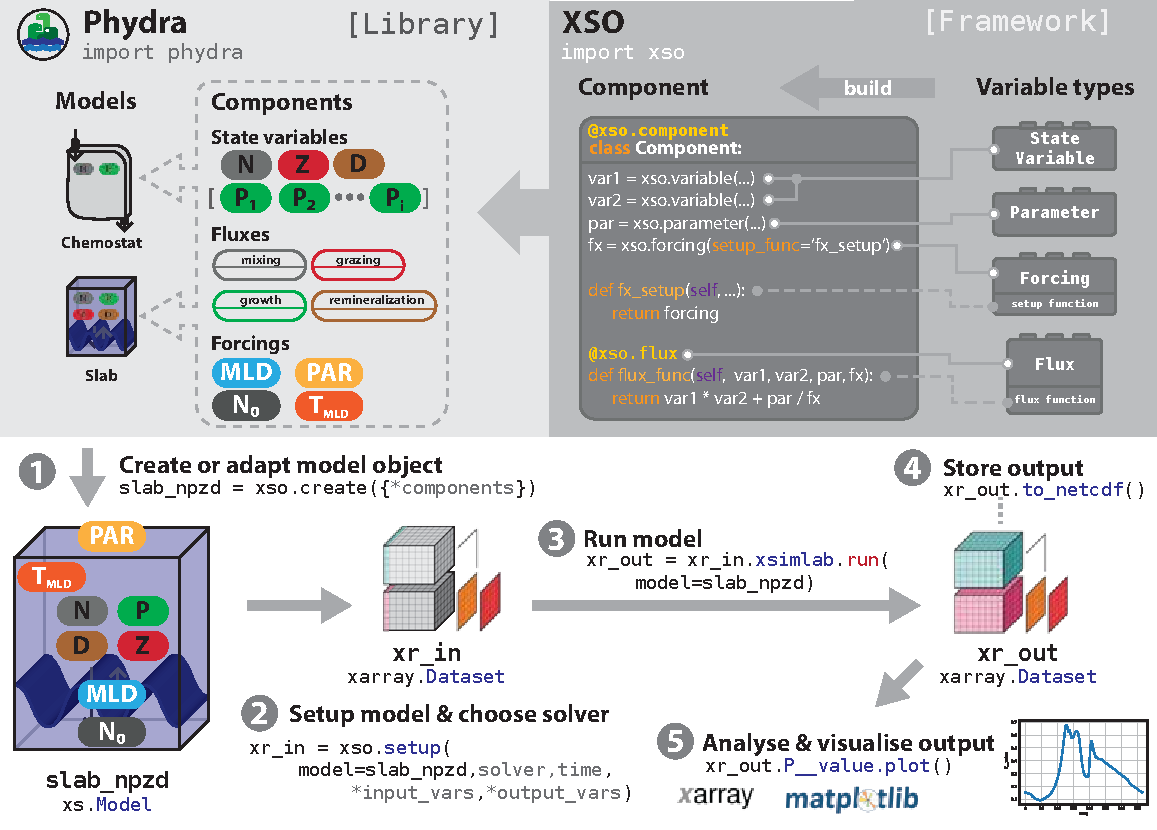
\includegraphics[width=12cm]{Figures/firstdraft_schematics/00_schematics_Package.pdf}
\caption{Schematic of package structure. XSO provides the framework. Phydra is a library of functional \textit{components} and pre-built \textit{model objects}, that can be used, extended, and modified. A typical workflow would consist of five steps. (1) Choose a pre-existing model, modify a model, or create a new model from components. (2) The model is setup with correct labels and parameters and a solver is chosen. (3) The model is run, all input and output data are contained in Xarray datasets. (4) Data are stored or shared. (5) Model output is returned as a "filled" Xarray dataset that is fully compatible to be analysed and visualised with the wealth of tools provided by the Python scientific ecosystem. The workflow is presented in detail in section \ref{Section:ModelDevelopmentWorkflow}.}
\label{Figure:PhydraXSOPackageSchematics}
\end{figure*}

% 2nd Section: 
% Background, theoretical framework. Specifics here!
The structure and functionality of Phydra and XSO and a simplified model development workflow are presented in Figure \ref{Figure:PhydraXSOPackageSchematics} and explained in more detail below. Interested researchers and potential users can find the most up-to-date documentation and code on GitHub (XSO: \url{https://github.com/ben1post/xarray-simlab-ode}, Phydra: \url{https://github.com/ben1post/phydra}). The documentation includes short guides on setting up a functional Python environment, including Jupyter Notebooks.

\subsection{The XSO framework} \label{Section:XSOFramework}

% 2.3 The simulation framework
% To organize and execute simulations, our environment is based on the Python library xarray-simlab (Bovy et al. 2021), a feature-rich and robust extension to the xarray library.

%The xarray-simlab library provides a framework to compose complex computational models from sets of reusable components, called processes. A collection of processes can be combined to form a model, and their computational ordering is entirely deduced from process dependencies. In essence, those dependencies are created by explicitly linking processes via output variables (producing processes) and input variables (consuming processes). Variables declared within a process class may be annotated with other useful metadata like unit, description, validation functions or specific encoding settings. The set of variables declared inside a process class describes the process interface in terms of computed variables. They may be consumed by any other process in the model as long as no circular dependencies are created. However, circular dependencies are allowed if a variable is consumed with an offset over time, i.e. in the following simulation step. For the case of interdependent variables, their evolution should be estimated within a common process, for example, using an appropriate numerical solver.

%The model—the predefined collection of processes—can be dynamically altered by plugging in or unplugging other processes, or by replacing a particular process with an alternative implementation. Processes may inherit from a base process class, and derived classes may implement a different model logic and provide additional output variables. Models and their processes and variables can be programmatically inspected, and the computational order, i.e. process dependency, can be easily visualized.

%In order to execute a particular model, users create a model set-up in which they define the basic parameters for each simulation run. The most important are the time steps, the values of the model input variables and the name of the variables to be exported.

%The xarray-simlab library provides great freedom in the design of a model and numerous ways to declare variables. We decided to separate three types of numerical data: pure constants like natural physical constants that are kept directly inside a Python module, variables that effectively vary during a simulation, and parameters that are either obtained from the literature or after a calibration process and are therefore constant within a simulation set-up. Each individual process may be parameterized with these separate files stored in the toml format. By default, an initialization function is associated with each process to load those parameter files and parameterize a process at startup. However, it is still possible to inject custom parameter values by reimplementing a process initialization function.

%Simulation inputs and outputs are mostly composed of xarray data structures (i.e. labelled arrays and data sets). All features from xarray are therefore readily available for all input and output data: index- and label-based selections; interpolation and grouping of data; reshaping and combining data sets; reading and writing files; and advanced plotting.

%To adapt this framework to FSPMs, we have extended the library with new features. L-systems models can be automatically integrated as processes, and the simulation runs with associated visualization (see following Section 2.4 below). While FSPMs simulate structures with a growing number of elements, xarray-simlab is originally designed to model the dynamics of structures with a fixed number of elements. We extended it so that all property arrays are automatically and consistently resized when new entities are created. The growth of the entity index over time does not make it possible to use xarray-simlab built-in parallelism capabilities. We therefore reimplemented the parallel processing of multi-model simulations using Python’s standard multiprocessing library. Our solution is not as efficient as some GPU-based solutions for L-systems (Lipp et al. 2010), but it offers great flexibility and expressiveness to define modelling processes thanks to Python and its scientific ecosystem.

%%%%%%%%%%%%%%%%%%%%%%%%%%%%%%%%%%%%%%%%%%%%%%%%%%%%%%%%%%%%%%%%%
% WHAT ABOUT DIMENSIONALITY? This is a big feature, not mentioned once...
%Mention dimensionality

% the following 2 paragraphs were copied from discussion, but actually belong in INTRO:
% Highlight (collaborative) modelling workflow
%The software presented here was designed to support collaborative model development. Scientists working with computational models do not always build the models themselves. Often, scientists use existing models and focus the work on parameterisation and analysis of results obtained with model applications to specific locations. This type of use is specifically supported in our software because we equipped the Phydra library with pre-built \textit{model objects} and \textit{components}. A user can start working with models without detailed knowledge of the underlying framework and learn the basic workflow before progressing to building custom models using the XSO framework. Additionally, more advanced users can easily share custom \textit{components} or \textit{model objects} via the respective Python objects. This particular design makes our software suitable for teaching. 
%!!!!Say how this might be done, and in what settings, with what equipment (e.g, a laptop or tablet).!!!!

% Highlight flexible dimension setup, great for testing PFT-type or allometry based models
%<Add a topic sentence.> An ecosystem model tracks chemical compounds as well as organisms via state variables. These state variables can define completely different components of a model, or represent a functional group. \textit{Components} within Phydra are defined at this higher level and can contain a single state variable or an array of state variables that share common fluxes with differing parameterisation that can be supplied as arrays at model setup. In the third model application, we presented such a case by using multiple state variables for phytoplankton and zooplankton as defined by size-based allometric functions. In addition to size, the \textit{components} and contained \textit{variable types} could be modified to include information on units or other parameters relevant to the model. The added flexible dimensionality of components was designed with the current issues in marine ecosystem model in mind. The effects of different levels of complexity in the number and definition of phytoplankton functional types (PFT), for example, is not routinely tested in marine ecosystem models. Phydra provides a framework that allows for easy testing through flexible modification of such model complexity at model setup.


Xarray-simlab-ODE (XSO) is a Python framework that allows you to construct and customize models based on ordinary differential equations (ODEs). XSO was developed as the technical foundation of the Phydra library, but is not limited to any particular domain and can used to create ODE-based models of any type.

The XSO framework is an extension of Xarray-simlab \citep{Bovy2018Xarray-simlab:Interactively}, which provides a generic modeling framework in Python. XSO extends this with functional building blocks and a solver backend for differential equation based models. It inherits the data structure, storing model input and output as Xarray data sets, which can be easily stored and shared, as well as further analysed using Xarray's built-in compatibility with the Python scientific ecosystem \citep{Hoyer2017Xarray:Python}. This allows users to easily document the full model development workflow and exchange and interact at multiple stages of the modelling process. XSO provides an interface for iterative modifications, both to more complex and simpler model constructs. The typical steps of a model development are presented in further detail in section \ref{Section:ModelDevelopmentWorkflow}.

% The following is too technical:
%XSO was designed following the object-oriented paradigm. The backend code is structured into a \textit{core} class that provides an interface between a model backend and an extensible solver class. As an open-source project, this backend code is openly accessible and was constructed to allow advanced users to extend functionality and provide custom solver implementations. Basic usage of XSO does not require any interaction with the backend, as all functionality is wrapped in custom attributes and decorators provided to construct \textit{components} (see section \ref{Section:CreatingXSOComponent}). 


The logical units of the XSO framework are listed below:
% I need to make this less technical as well, just mention the very basics.
\begin{itemize}
    \item  \textit{Variable types}. These are the most basic element of a model. XSO provides a set of \textit{variable types} that can be used as attributes or function decorators when constructing \textit{components}. XSO currently provides the following attributes: \textit{variable}, \textit{forcing}, \textit{parameter}, \textit{flux} or \textit{group}.  % TOO TECHNICAL?: The class decorator \texttt{@xso.component} converts the \textit{variable types} to functional Xarray-simlab variables and registers them within the model backend. These variable types are explained in greater detail in section \ref{Section:CreatingXSOComponent}.
    
    \item \textit{Components}. These are the logical building-blocks of a computational model that declare a subset of variables used in the model and defines a specific set of mathematical functions computed for these variables during model runtime. More specifically, a \textit{component} refers to a Python class containing \textit{variable types} that is decorated with the \texttt{xso.component} function. For example, a \textit{component} could define a specific nutrient uptake function, e.g. Monod-type phytoplankton growth on a single nutrient. The decorating function registers the \textit{variable types} within the framework, reducing boilerplate code and creating fully functional model building blocks. 
    %The XSO framework provides a collection of custom attributes (i.e. \textit{variable types}) that can be flexibly combined into a single \textit{component}. \textit{Components} can contain any number of variable types and functions. Linking variables between \textit{components} occurs at model setup via the supplied labels.
    
    \item \textit{Model object}. These are instances of the Model class provided by Xarray-simlab. They consist of an ordered, immutable collection of \textit{components}. A XSO \textit{model object} is created with a call to the function \texttt{xso.model()} by supplying a dictionary of model \textit{components} with their respective labels. XSO provides an interface for running pre-built \textit{model objects} that contain all \textit{components} relevant to the model. These can be easily stored and shared to users not proficient in model construction that are interested in using a specific model with custom parameterisation.
    
    \item \textit{Model setup}. This object is an Xarray dataset, that includes all relevant information needed at runtime and provides custom methods via Xarray-simlab. When executing the model by calling the \texttt{xsimlab.run()} method of the \textit{model setup} and supplying the appropriate \textit{model object}, a "filled-out" Xarray dataset is returned containing model setup parameters, metadata and output. Additionally a \textit{model setup} provides methods for updating only specific parameters or supplying multiple sets of parameters in a batch dimension. When supplying the batch dimension at model runtime, the model is solved for each set of parameters along the dimension and returned as a single Xarray dataset with labelled dimensions. Similarly to \textit{model objects}, \textit{model setups} can be readily stored and shared.
\end{itemize}


% DON'T REPEAT YOURSELF OVER AND OVER !
% Mention limitiation
% But highlight the flexibility and benefits
The XSO framework is currently limited to model applications based on ordinary differential equations (ODEs). With this limitation, conceptual marine ecosystem models still vary greatly in complexity. Our objective in developing the XSO framework was to enable users to construct ODE-based models of any complexity, particularly in regards to the number of state variables and processes involved. This was achieved by providing \textit{variable types} which correspond directly to the fundamental mathematical components of ODE-based models (e.g. state variables, parameters, forcing, and partial equations). All aspects of the model must be defined at the level of \textit{variable types}. The \textit{components} of the model can be freely assembled from the available \textit{variable types}, allowing the user to wrap a logical component of the model as desired. Apart from the technical limitations of the solver algorithm used, there are no restrictions on the number of \textit{variable types} used within a \textit{component} and no limitations to the levels of \textit{group} variables linking components to define a single ecosystem process. 

State variables, forcing, and parameters must be initialized in one \textit{component} and can be referenced throughout the model. The system of differential equations is constructed from the \textit{fluxes} within the \textit{components} using the labels supplied during model setup. The number of values in a defined dimension is flexible, and \textit{group} variables can provide flexible linkages and number of terms between \textit{components}. These design choices ensure that the effort required to construct a model is proportional to the desired level of complexity, models and \textit{components} can be easily modified to incorporate more complex formulations. We hope that this will encourage experimentation and inter-comparison of model performance across a range of complexities.

% SOLVER
XSO currently provides two solving algorithms: an adaptive step size solver from the SciPy package (odeint) and a simple stepwise solver that is built into the backend Xarray-simlab framework.

% Computational Efficiency




\subsection{The Phydra library} \label{Section:PhydraLibrary}
Phydra is python package, that provides a library of marine ecosystem models built in a modular fashion using the XSO framework. The Phydra package provides a specific library for marine ecosystem modelling applications that establishes conventions and common usage.

 
The marine ecosystem models included in the Phydra package are available to the user at multiple hierarchical levels: as a library of pre-built XSO model \textit{components}, as pre-assembled \textit{model objects}, and as exemplary model simulations in interactive Jupyter notebooks.
These levels are described below.

\begin{enumerate}
    \item \textit{Components}. The first version of the library will contain all \textit{components} used to create the three model applications presented in Section \ref{Section:UseCases}. The \textit{components} can be combined to zero-dimensional marine ecosystem models of variable complexity. The library follows common usage patterns and conventions. As long as the labelled model dimensions between \textit{components} match at model setup, all \textit{components} included in the Phydra library are compatible.
    
    \item \textit{Model objects}. The first release of phydra contains the \textit{model objects} defined in the three model applications presented in section \ref{Section:UseCases}. The \textit{model objects} can be imported from the library and can be setup, modified, and run by a user.
    
    \item \textbf{Example notebooks}: \textit{Model objects} only define the collection of \textit{components} for a specific model implementation. Phydra comes with one fully documented model application per \textit{model object} that is presented in an interactive Jupyter notebook. These notebooks show all steps from creating the \textit{model setup} object to analysing model output and provide a template for further exploration and experimentation with the provided marine ecosystem models.
    
\end{enumerate}

The open-source and extensible nature of Phydra and XSO enables users to customize and develop processes that accurately describe a particular ecosystem. In a collaborative effort to promote efficient, transparent, and reproducible marine ecosystem modeling, Phydra encourages users to contribute their own \textit{components} and \textit{models} to the core library. The Phydra library could potentially offer a comprehensive, well-documented, and peer-reviewed codebase for the scientific exploration of marine ecosystem models.

\subsection{Workflow for developing a model from pre-built components} \label{Section:ModelDevelopmentWorkflow}

We illustrate here the key steps of configuring and running an ecosystem model using the XSO framework. The workflow is presented in Figure \ref{Figure:PhydraXSOPackageSchematics}.

\begin{enumerate}
% this needs to be more user workflow, less backend explanation (leave that to previous framework explanation), instead focus on the actual functions and arguments, step by step
    \item  \textbf{Creating a \textit{model object}:} 
    A typical modelling workflow would begin with a \textit{model object}. The \textit{model object} can be imported from the Phydra library or assembled from the provided \textit{components}. The procedure for creating custom \textit{components} is explained in section \ref{Section:CreatingXSOComponent}. A \textit{model object} is created by calling the function \texttt{xso.model()} with a single argument: \texttt{model\_dict}. This argument is a dictionary of model \textit{components} with their respective labels. The supplied labels identify the \textit{components} for all future steps. The function call automatically includes processes handling model assembly and the solver backend. When creating a model, the XSO framework automatically orders the processes in their logical order of execution and returns the \textit{model object}. The user can interactively view all parameters required as input at model setup by printing the object in the console.

    \item \textbf{Creating a \textit{model setup}:} The next step is to create a \textit{model setup} corresponding to the \textit{model object}. The \textit{model setup} object is an Xarray dataset that contains all provided parameters as well as the initialized labelled model dimensions and supplied metadata. It is created with a call to \texttt{xso.setup()} by supplying the following arguments:
    \begin{itemize}
        \item \texttt{model}. This argument takes the \textit{model object} created in the previous step. It provides the blueprint for the \textit{model setup} and the backend checks \textit{components} and variable labels against the provided \textit{model object}.
        \item \texttt{solver}. The solver can be chosen from those implemented in the XSO backend via the appropriate string label. Additionally, the user can supply a custom solver implementation based on the abstract solver base class available within the XSO framework.
        \item \texttt{input\_vars}. In order to fully initialize a model that can be solved, a user needs to supply a complete set of parameters and labels linking forcing and variables between \textit{components} to the \texttt{input\_vars} argument. The argument takes a dictionary where each component is referenced via the label supplied when the \textit{model object} was created. The parameters and variables are referenced via the attribute names defined when creating the \textit{component}. Multiple values for a specific parameter can be passed with an additional batch dimension. At model runtime the model can be solved for each set of parameters within the batch dimension.
        \item \texttt{output\_vars}. The user can specify output variables, by default (if no input is provided) all values of variables, forcing and fluxes are stored after model runtime.
        \item \texttt{time}. To specify the time-steps used for model execution, the user has to supply an array of time steps. The array can be created using Numpy functions such as \texttt{linspace} and is then passed  to the \texttt{time} argument.
    \end{itemize}
    At this stage the user can store the fully initialized \textit{model setup} for later use or for sharing with other users.
    
    \item \textbf{Running model simulations:} The \textit{model setup} created in the previous step contains all necessary information needed at model runtime. All that is required of the user at this stage is to call the \texttt{xsimlab.run()} method and provide a model object corresponding to the model setup. The runtime method is provided by the underlying Xarray-simlab framework with the following arguments.
    \begin{itemize}
        \item \texttt{model}. This argument takes the \textit{model object} created in the previous step.
        \item \texttt{batch\_dim}. If defined at model setup, the label of the batch dimension has to be supplied to the \texttt{batch\_dim} argument.
    \end{itemize}
    The method returns model outputs as a new Xarray dataset, which can be used in the following steps.
    
    \item \textbf{Storing model output:} Simulation inputs and outputs can be kept in memory or saved on disk. The \texttt{to\_netcdf()} method stores the full model outputs including metadata and labelled dimensions to a NetCDF file at a location specified by the user.
    
    \item \textbf{Analyzing and visualizing model output:} The Xarray dataset created at model runtime is natively compatible with a wealth of packages for data analysis and visualization from the Python scientific ecosystem. Xarray provides built-in compatibility with the standard plotting library Matplotlib and more advanced data-visualization tools like Hvplot that make full use of the labelled dimensions for plotting multidimensional data. The data for a specific dimension can be extracted to Pandas data-frames (a popular package for data analysis) via the \texttt{to\_dataframes()} method. Specific variables can be indexed and extracted as Numpy arrays via their \textit{component} and variable labels. These methods provide a rich interface and full compatibility with advanced data analysis tools created by the open-source Python community.

\end{enumerate}


 %% \ SECTION 3
\section{Model applications} \label{Section:UseCases}

To showcase the utility of the XSO framework, we present three marine ecosystem model applications of varying complexity. For each application we present the mathematical model, the implementation within the XSO framework and model results. To highlight the modular nature of the framework, we also show how one aspect of each model is modified.

For the first model application, we considered a highly simplified model, whose implementation is presented in full detail. To simplify the presentation of the more complex models in use cases 2 and 3, we show only the component structure and highlight additional technical aspects of the implementation. For all use cases the complete code, following the full model development workflow from model creation to output visualization, is available publicly as interactive Jupyter notebooks in the Phydra repository (\url{https://github.com/ben1post/phydra/tree/master/examples}).

\subsection{Model application 1: phytoplankton growth in a chemostat}
%%f
\begin{figure}[t]
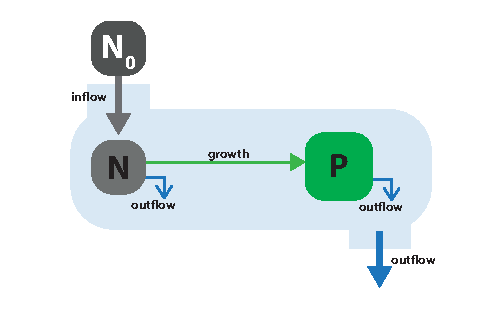
\includegraphics[width=8.3cm]{Figures/firstdraft_schematics/01_schematics_Chemostat.pdf}
\caption{Schematic of model application 1: phytoplankton $P$ feeding on a single nutrient $N$ in a flow-through system. The chemostat system includes an external nutrient input with concentration $N_0$. Both $N$ and $P$ flow out of the system at a constant dilution rate, $d$.}
\label{Figure:ModelSchematics_1}
\end{figure}

The first model we present, is a model of a phytoplankton population growing in a chemostat. Chemostats are a commonly used experimental setup for studying the dynamics of microorganisms under controlled laboratory settings. They are characterized by constant influx of medium containing nutrients and a constant outflow of the culture, with a rate of $d$ (units). This allows the implementation of steady-state system, that is particularly useful for studying the growth dynamics of microorganisms. Although the conditions of chemostat systems do not have an equivalent in nature, some oceanic upwelling systems can be approximated with such a simple model \citep{Haefner2005ModelingApplications}.

To showcase the flexibility and simplicity of the XSO framework, we considered two cases: (1) a constant nutrient input and (2) a sinusoidal nutrient input.

\subsubsection{Description}
The model is presented in Figure \ref{Figure:ModelSchematics_1}. It uses nitrogen as its currency (quantities are measured in units of $\mu mol$ N $m^{-3}$, or $\mu M$), with state variables for dissolved nutrients ($N$) and phytoplankton ($P$). The physical environment is a flow-through system corresponding to a laboratory chemostat setup. Growth medium with nutrient concentration $N_0$ flows into the system at a rate $d$. The model components ($N$ \& $P$) flow out of the system at that same rate.

Phytoplankton growth ($\mu$) is described by Monod kinetics \citep{Monod1942RecherchesBacteriennes}.
\begin{equation}
    \mu = \mu_{max} \frac{N}{k + N} 
\end{equation}
where $k$ is the half-saturation nutrient concentration, defined as X, $N$ is the ambient nutrient concentration, and $\mu_{max}$ is the maximum growth rate achievable under perfect growth conditions.

The model equations are:

\begin{equation}
    \frac{d N}{d t} = 
    d (N_0 - N) % Nutrient input and output
    -  \mu_{max} \frac{N}{k_N + N} 
\end{equation}

%PHYTOPLANKTON
\begin{equation}
    \frac{d P}{d t} =
    \mu_{max} \frac{N}{k_N + N} 
    - d P
\end{equation}



\subsubsection{Implementation}

%%f
\begin{figure*}[t]
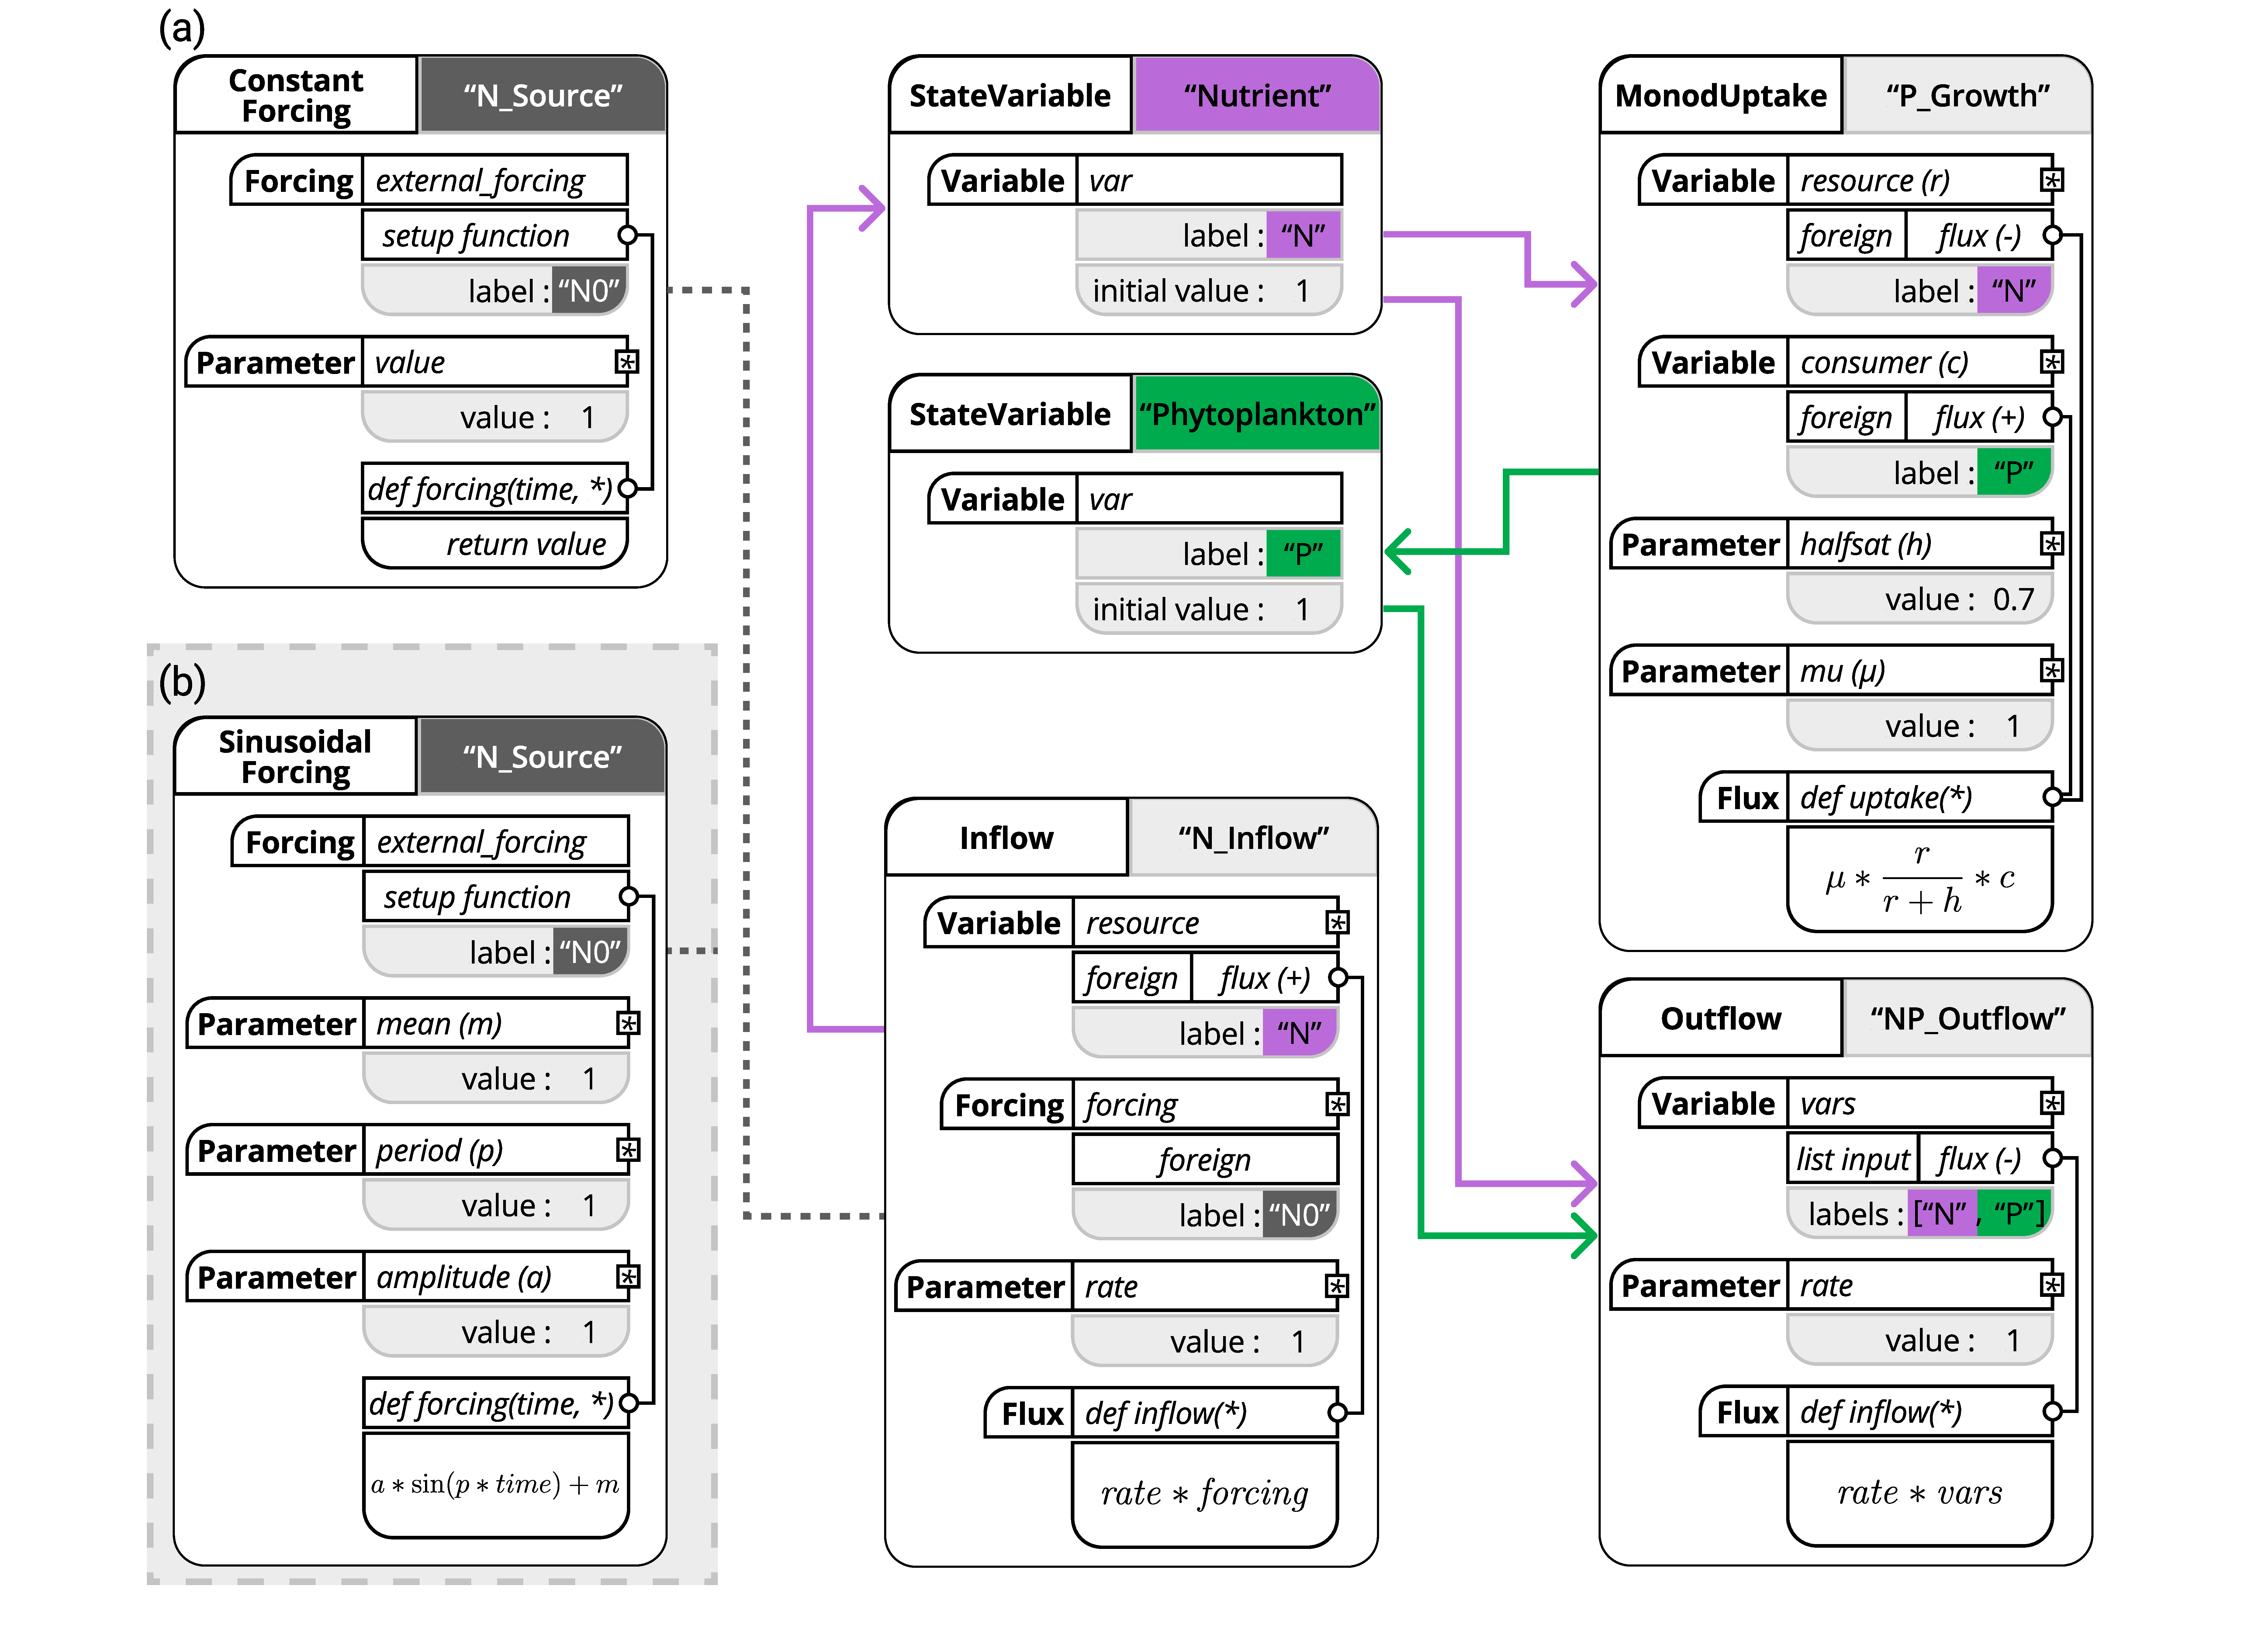
\includegraphics[width=15cm]{Figures/firstdraft_schematics/code_schematics/Chemostat.pdf}
\caption{A schematic representation of how model application 1 is implemented in the XSO framework and included in the Phydra library. Model setup with constant forcing (a) and with sinusoidal forcing (b). Structures in solid black are hard-coded into components. Labels of the different components are supplied at model creation. Gray boxes and the resulting links between components (shown as thick coloured arrows and dashed lines) are defined at model setup, via the supplied labels and parameters. The asterisk in the flux function input arguments references the variables, forcing and parameters defined within the same component, these local variables can be used in all functions (e.g. fluxes or forcing setup functions) within that same component.}
\label{Figure:CodeSchematics_1}
\end{figure*}

In order to find a useful structuring of model components, we can separate the model into state variables, forcing, and fluxes. For state variables, we have nutrient ($N$) and phytoplankton ($P$). The only forcing is the nutrient concentration of the external medium ($N_0$), whether it is constant or variable. Three fluxes can be separately defined: (1) the inflow of the external medium, (2) $P$ growing on $N$, and (3) the outflow of both $N$ and $P$.
The model was implemented using these 6 separate model components, as visualized in Figure \ref{Figure:CodeSchematics_1}.

The model implementation and structure built from Phydra components is presented in detail in appendix \ref{Appendix:Implementation1}.


%%% TWO-COLUMN TABLE
%
%t
\begin{table*}[t]
\caption{Model parameters used in application 1.}
\begin{tabular}{l c c r}
\tophline
Parameter & Description & Value & Units \\
\middlehline

$N_0$ & nutrient concentration of external medium & 0.1 & \unit{µM \ N} \\
$\mu_{max}$ & maximum growth rate & 1 & \unit{d^{-1}} \\
$d$ & dilution rate & 0.1 & \unit{d^{-1}}\\
$k_N$ & half-saturation nutrient concentration & 0.7 & \unit{µM \ N}\\

\bottomhline
\end{tabular}
\label{Table:UseCase1Parameters}
\end{table*}
%

To explore the basic dynamics, we chose standard parameters values (Table \ref{Table:UseCase1Parameters}). Initial values for $N$ and $P$ were set at 1 (units) and 0.1 (units), respectively. The model was run for X days with a time step of Z.

In order to run the model with periodic forcing, we can simply exchange the forcing component from \texttt{ConstantForcing} to \texttt{SinusoidalForcing}. This specific component requires more input parameters, but otherwise the model creation and setup remain the same. There is also the option to update the pre-existing model object and model setup object by simply supplying the \texttt{SinusoidalForcing} component for the \texttt{"N\_inflow"} component via the \texttt{model.update\_processes()} method and updating the corresponding parameters via \texttt{model\_setup.update\_vars()} functions supplied by the Xarray-Simlab framework that XSO extends. Such functionality allows straightforward modification and testing of models.

\subsubsection{Results}

%%f
\begin{figure}[t]
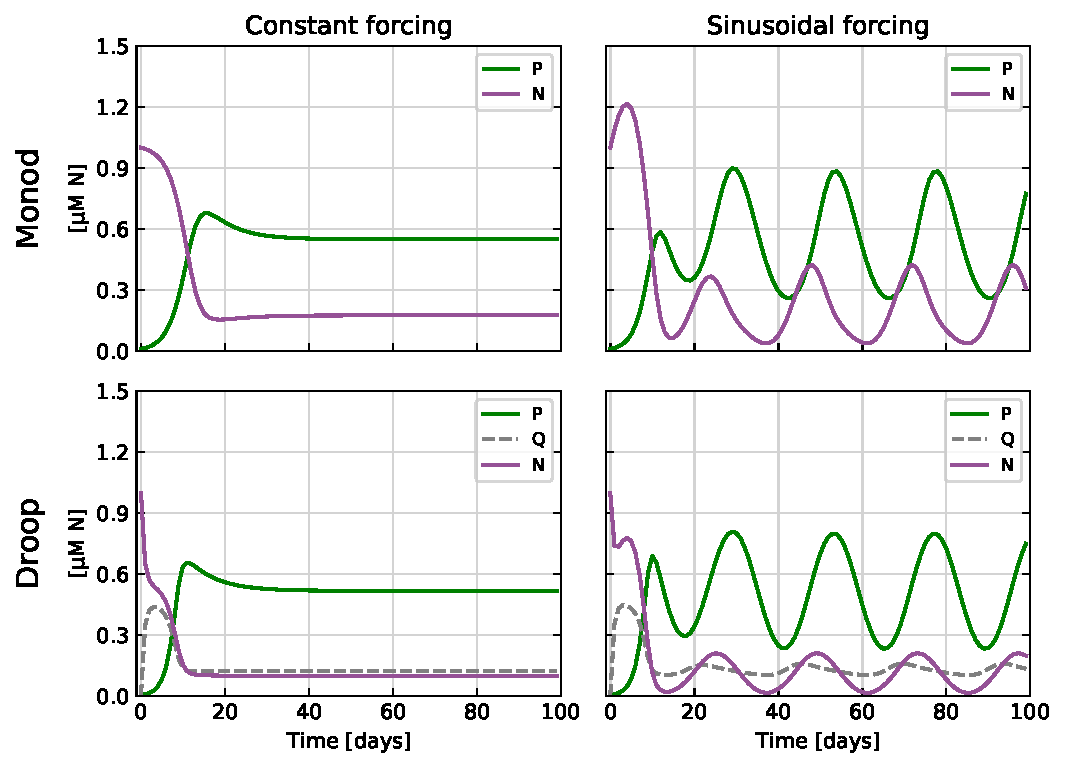
\includegraphics[width=8.3cm]{Figures/firstdraft_plots/01_chemostat_output.pdf}
\caption{Model output for the two chemostat model scenarios: (a) Constant forcing and (b) Sinusoidal forcing. In each case, the concentration of nutrient (N; color) and phytoplankton (P; color) are shown through time.}
\label{Figure:ResultsChemostat}
\end{figure}

Figure \ref{Figure:ResultsChemostat} shows the results of the two model runs, with constant nutrient concentration and with periodically variable external nutrient concentration. With the constant forcing, the model quickly reaches a steady state, as nutrient supply and the resulting phytoplankton growth balances with the loss of nutrient and phytoplankton due to the constant outflux of medium. The periodically variable nutrient concentration creates oscillations in $P$ centred around 0.9 \unit{µM \ N}).

This first model application represents a basic proof-of-concept that our presented library and framework can create expected results within a very simple model setup.

\subsection{Model application 2: NPZD slab model}
%%f
\begin{figure}[t]
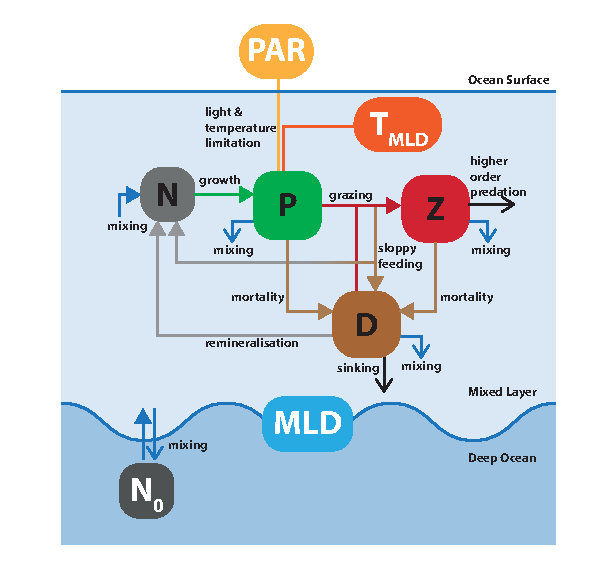
\includegraphics[width=8.3cm]{Figures/firstdraft_schematics/02_schematics_EMPOWER.pdf}
\caption{Model schematic of the Nutrient-Phytoplankton-Zooplankton-Detritus (NPZD) slab model presented as a second application. The model structure is adapted
from \citet{Anderson2015c}. Boxes with black and white fonts represent state variables and external forcing, respectively. Arrows indicate fluxes between state variables. The upper layer box contains the ecosystem model. The curvy blue line represents the variable mixed layer depth that defines the boundary between the upper layer and the inert deep ocean. Briefly state what you mean by "slab"}
\label{Figure:ModelSchematics_2}
\end{figure}

The second application describe a classic Nutrient-Phytoplankton-Zooplankton-Detritus, or NPZD, model embedded in a slab-ocean physical setting \citep[e.g.,][]{Evans1985ACycles, Fasham1990a}. The simplified two-layer structure provides a simple zero-dimensional description of physical processes affecting plankton ecosystems in the open ocean. This classic model structure constitutes an efficient physical setting for more complicated ecosystem descriptions and is often used for teaching marine ecosystem modelling \citep{Anderson2015c}. The presented application is an implementation of the EMPOWER model, as presented by \citet{Anderson2015c}. See Figure \ref{Figure:ModelSchematics_2} for a schematic of the model structure. <Briefly describe the ecosystem, ie "Model phytoplankton growth is tied to temperature, light, and nutrients, phytoplankton are consumed by zooplankton predaors, etc">

The published model code was written as an R script, with some modifications allowed via user supplied flags. We updated the model code to the modular and flexible XSO framework, allowing for greater adaptability and experimentation on this classic structure.

Many NPZD-type models have been published over the years, with many different formulations for the functional responses of the ecosystem components. The EMPOWER model was presented with various formulations for the treatment of light. We followed the same approach by considering two different light-attenuation algorithms that can be easily exchanged in the modular framework.

\subsubsection{Description}
% for EMPOWER move all description to supplementary, no need to explain everything again
% use simple plain english paragraph describing model
The model uses nitrogen as currency (quantities are measured in units of $\mu mol$ N $m^{-3}$), with state variables for dissolved nutrients ($N$), phytoplankton ($P$), zooplankton ($Z$) and detritus ($D$). The water column is represented by two layers, where a biologically inert deep ocean box is situated below a homogeneously mixed upper box of variable depth that contains the ecosystem. The model structure, locations, and parameters are adapted from the EMPOWER model \citep{Anderson2015c}.

The model is driven by external forcing describing the depth of the upper mixed layer ($H$; units), average temperature of the upper mixed layer ($T$; units), photosynthetically active radiation (PAR) at the surface ($I$; units), and nutrient concentration in the deep layer ($N_0$; units). 

% Nutrient dynamics
The deeper layer supplies nutrients to the upper layer, while other components are mixed to the deep layer and lost from the system. The magnitude of mixing is described by $K$ (units):

\begin{equation}
    K = \frac{h^{+} + \kappa}{H}
\end{equation}

Where $\kappa$ (units) represents constant diffusive mixing. Variable mixing is a function of the change in mixed layer depth (MLD) over time $h = \frac{dH}{dt}$. The function $h^{+}$ defines the effects of entrainment and detrainment due to the changes in MLD as $h^{+} = \max(0, \ h)$. When the mixed layer shallows, $h^{+}$ does not modify $K$, based on the assumption that detrainment of mass and the increase in concentration due to the reduced volume of the mixed layer are balanced \citep{Evans1985ACycles}. 

%\subsubsection{Nutrients}
Dissolved nutrients in the mixed layer ($N$) are supplied via mixing, a fraction of zooplankton excretion, and remineralization of detritus. Nutrients are entrained from the bottom layer. Mixing of nutrients is a positive term, adding to $N$ according to the sign of the gradient between $N_0$ and $N$. The general direction of the nutrient flux is from a variable and nutrient-rich bottom layer to the upper layer. This nutrient flux supports phytoplankton growth, which is the only loss term for $N$.

%\subsubsection{Phytoplankton}
The growth rate of phytoplankton $P$ ($\mu_{P}$) is the product of a temperature-dependent maximum growth rate ($\mu_P^{max}(T)$) and the growth-dependencies on light ($\gamma^{I}$) and nutrients ($\gamma^{N}$): 

\begin{equation}
    \mu_{P} = \mu_P^{max}(T) \ \gamma^{I} \ \gamma^{N}
\end{equation}

$T$ is the temperature of the upper mixed layer in \unit{\degree C}, as supplied from external forcing. Under the assumption of balanced growth, the maximum growth rate of phytoplankton $\mu_P^{max}(T)$ is equivalent to the temperature-dependent maximum photosynthetic rate $V_P^{max}(T)$. The function is parameterized via the maximum photosynthetic rate at 0 \unit{\degree C}, represented as $V_P^{max}(0)$. Temperature dependence is calculated via the Eppley curve \citep{Eppley1972TemperatureSea}.

\begin{equation}
    V_P^{max}(T) = V_P^{max}(0) \ 1.066^T
\end{equation}

Nutrient limitation of phytoplankton growth $\gamma^N$ is described by the Michaelis-Menten growth kinetics.

\begin{equation}
    \gamma^N = \frac{N}{k_N + N}
\end{equation}

where $k_N$ is the half-saturation nutrient concentration. $N$ is the ambient nutrient concentration.

The term $\gamma_{I}$ represents growth-dependence on total light ($I$) available to phytoplankton through the whole upper mixed layer. We use the formulation of Smith (add citation) to calculate the photosynthetic rate:

\begin{equation}
    V_P = \frac{\alpha ~ I ~ V_P^{max}}{\sqrt{(V_P^{max})^2 + \alpha^2 I^2}}
\end{equation}

Where $V_P^{max}$ is the maximum photosynthetic rage, $\alpha$ is the slope of the P-I curve, and $I$ is irradiance.

$I$ decays exponentially with depth $z$ in the mixed layer:

\begin{equation}
    I(z) = I \ \exp{(-k_{PAR} \ z)}
\end{equation}

The attenuation coefficient $k_{PAR}$ is the sum of light attenuation due to water, $k_w$, and due to the presence of phytoplankton (self-shading), accounted for with a term proportional to the concentration of phytoplankton $k_c \cdot P$ (with $k_c$ constant of proportionality), thus:

\begin{equation}
    k_{PAR} = k_w + k_c \cdot P
\end{equation}

The numerical solution for the light-limitation on phytoplankton growth is calculated by combining the equations (give the numbers here) and integrating $I(z)$ through the upper mixed layer.

In addition to this standard light attenuation procedure, we also considered light attenuation according to a three-layer model of the upper mixed layer  \citep{Anderson1993APhotosynthesis}. This alternative formulation calculates multiple $k_{PAR, i}$, with i = 1 for the top 5 \unit{m}, i = 2 for the depth range 5 - 23 \unit{m} and i = 3 for depths below 23 \unit{m}. The changing spectral properties of water are taken into account by polynomial coefficients ($b_{0,i}$ to $b_{5,i}$).
\begin{equation}
    k_{PAR, i} = b_{0,i} + b_{1,i} C^{1/2} + b_{2,i} C + b_{3,i} C^{3/2} + b_{4,i} C^2 + b_{5,i} C^{5/2}
\end{equation}
where $C$ represents the pigment (chlorophyll) concentration. The values of the polynomial coefficients are given in the Appendix.

Non-grazing mortality of phytoplankton is described by the sum of linear $m_P$ and quadratic $m_{P2}$ factors \citep{Yool2011Medusa-1.0:Domain}. The former accounts for natural mortality and excretion. The latter describes higher order loss processes, including for example viral infection. All non-grazing phytoplankton loss terms feed into the detritus pool.

%\subsubsection{Zooplankton}
Zooplankton graze upon phytoplankton and detritus. The grazing function is a Holling Type 3 grazing response \citep{Anderson2015c}:

\begin{equation}
    G_P = \mu_Z \left( \frac{ \hat{\varphi}_P P}{(k_Z)^2 + \hat{\varphi}_D D +\hat{\varphi}_P P}  \right) Z
\end{equation}
where $\hat{\varphi}_P$ = $\varphi_P \ P$ and $\hat{\varphi}_D$ = $\varphi_D \ D$.

This formulation describes the total biomass of phytoplankton that is grazed $G_P$. Parameter $\mu_Z$ is the maximum ingestion rate of the food source, in this case both phytoplankton and detritus. The grazing preference parameters $\varphi_P$ and $\varphi_D$ do not represent a discrete fraction of the amount grazed in the diet relative to the environment. Instead, this amount is represented by the ratio of $\hat{\varphi}_P$ and $\hat{\varphi}_D$. 
The half-saturation constant for grazing $k_Z$ scales the density-dependent half-saturation constant $k_P$ for grazing on phytoplankton based on the choice of $\varphi_P$, with the relationship $k_P$ = $\sqrt{\frac{(k_Z)^2 }{\varphi_P}}$.

Grazing on detritus is defined as
\begin{equation}
    G_D = \mu_Z \left( \frac{ \hat{\varphi}_D D}{(k_Z)^2 + \hat{\varphi}_D D +\hat{\varphi}_P P}  \right) Z
\end{equation}

Zooplankton food ingestion does not directly convert into biomass. The total biomass grazed ($G_P + G_D$) is fractionated into zooplankton growth (to $Z$), excretion of dissolved nutrients (to $N$) and egestion of fecal matter \& particles (to $D$). Zooplankton growth is a product of total biomass grazed ($G_P$) and the gross growth efficiency (GGE) of zooplankton. The two parameters defining GGE in this model are absorption efficiency ($\beta$) and net production efficiency ($\epsilon$). Adsorption efficiency $\beta$ describes the fraction of $G_P$ that is absorbed in the gut, of which the fraction $\epsilon$ is actually assimilated into biomass (to $Z$: \ $\beta \epsilon$) and the rest is excreted as dissolved nutrient (to $N$: \ $\beta (1-\epsilon)$). GGE is the product of $\epsilon$ and $\beta$, for which values between 0.2 and 0.3 have been observed for a wide range of zooplankton \citep{Straile1997GrossGroup}. The fraction of $G_P$ egested to $D$ (e.g. as fecal pellets) is calculated via $1-\beta$. 

Similar to phytoplankton mortality, a linear mortality factor $m_Z$ represents natural mortality and excretion and feeds into the pool of detritus. A quadratic factor $m_{Z2}$ describes higher order predation on zooplankton, for example from fish, and is removed from the system. 

%\subsubsection{Detritus}
The detritus concentration in the upper layer ($D$) is supplied by mortality of phytoplankton, linear zooplankton mortality, and zooplankton egestion (e.g. fecal pellets). The loss terms are remineralization, grazing, mixing, and additional sinking. 

Detritus is remineralized at a constant rate $m_D$ to $N$. Similar to $P$ and $Z$, $D$ is affected by mixing through changes in MLD, described by the mixing coefficient $K$. In addition to $K$, detritus experiences losses due to gravitational sinking at a rate $v_D$. 

%\subsubsection{Model equations}
The rates of change of the state variables are described by the following set of equations. For the definition of all symbols used here see Table \ref{appendix:table:usecase1symbols} and see \citet{Anderson2015c} for a more detailed discussion of model structure and formulation.

%Nutrient
\begin{equation}
    \frac{d N}{d t} = 
    K (N_0 - N) % Nutrient mixing
    + \beta(1 - \epsilon)(G_P + G_D) % Unassimilated grazing by Z
    + m_D \ D % Remineralisation of D
    - \mu_{P} \ P % Phytoplankton gains
\end{equation}

%PHYTOPLANKTON
\begin{equation}
    \frac{d P}{d t} =
    \mu_{P} \ P  % Phytoplankton gains
    - m_P \ P % Linear mortality
    - m_{P2} \ P^2 % Quadratic mortality
    - G_P % Z grazing
    - K \ P % Phytoplankton mixing
\end{equation}

%ZOOPLANKTON
\begin{equation}
    \frac{d Z}{d t} =
    \beta \ \epsilon(G_P + G_D) % Assimilated grazing
    - m_Z \ Z % Linear mortality
    - m_{Z2} \ Z^2 % Quadratic mortality
    - K \ Z % Zooplankton mixing
\end{equation}

%DETRITUS
\begin{equation}
    \frac{d D}{d t} = 
    m_P \ P % Linear mortality
    + m_{P2} \ P^2 % Quadratic mortality
    + m_Z \ Z % Linear mortality
    + (1 - \beta)(G_P + G_D) % Unassimilated grazing by Z
    - G_D % Z grazing on D
    - m_D \ D % Remineralisation of D
    - K \ D % Mixing of D
    - \frac{v_D}{H} \ D % Sinking of D
\end{equation}


\subsubsection{Implementation}
% here present the implementation as is used in phydra

%%f
\begin{figure*}[t]
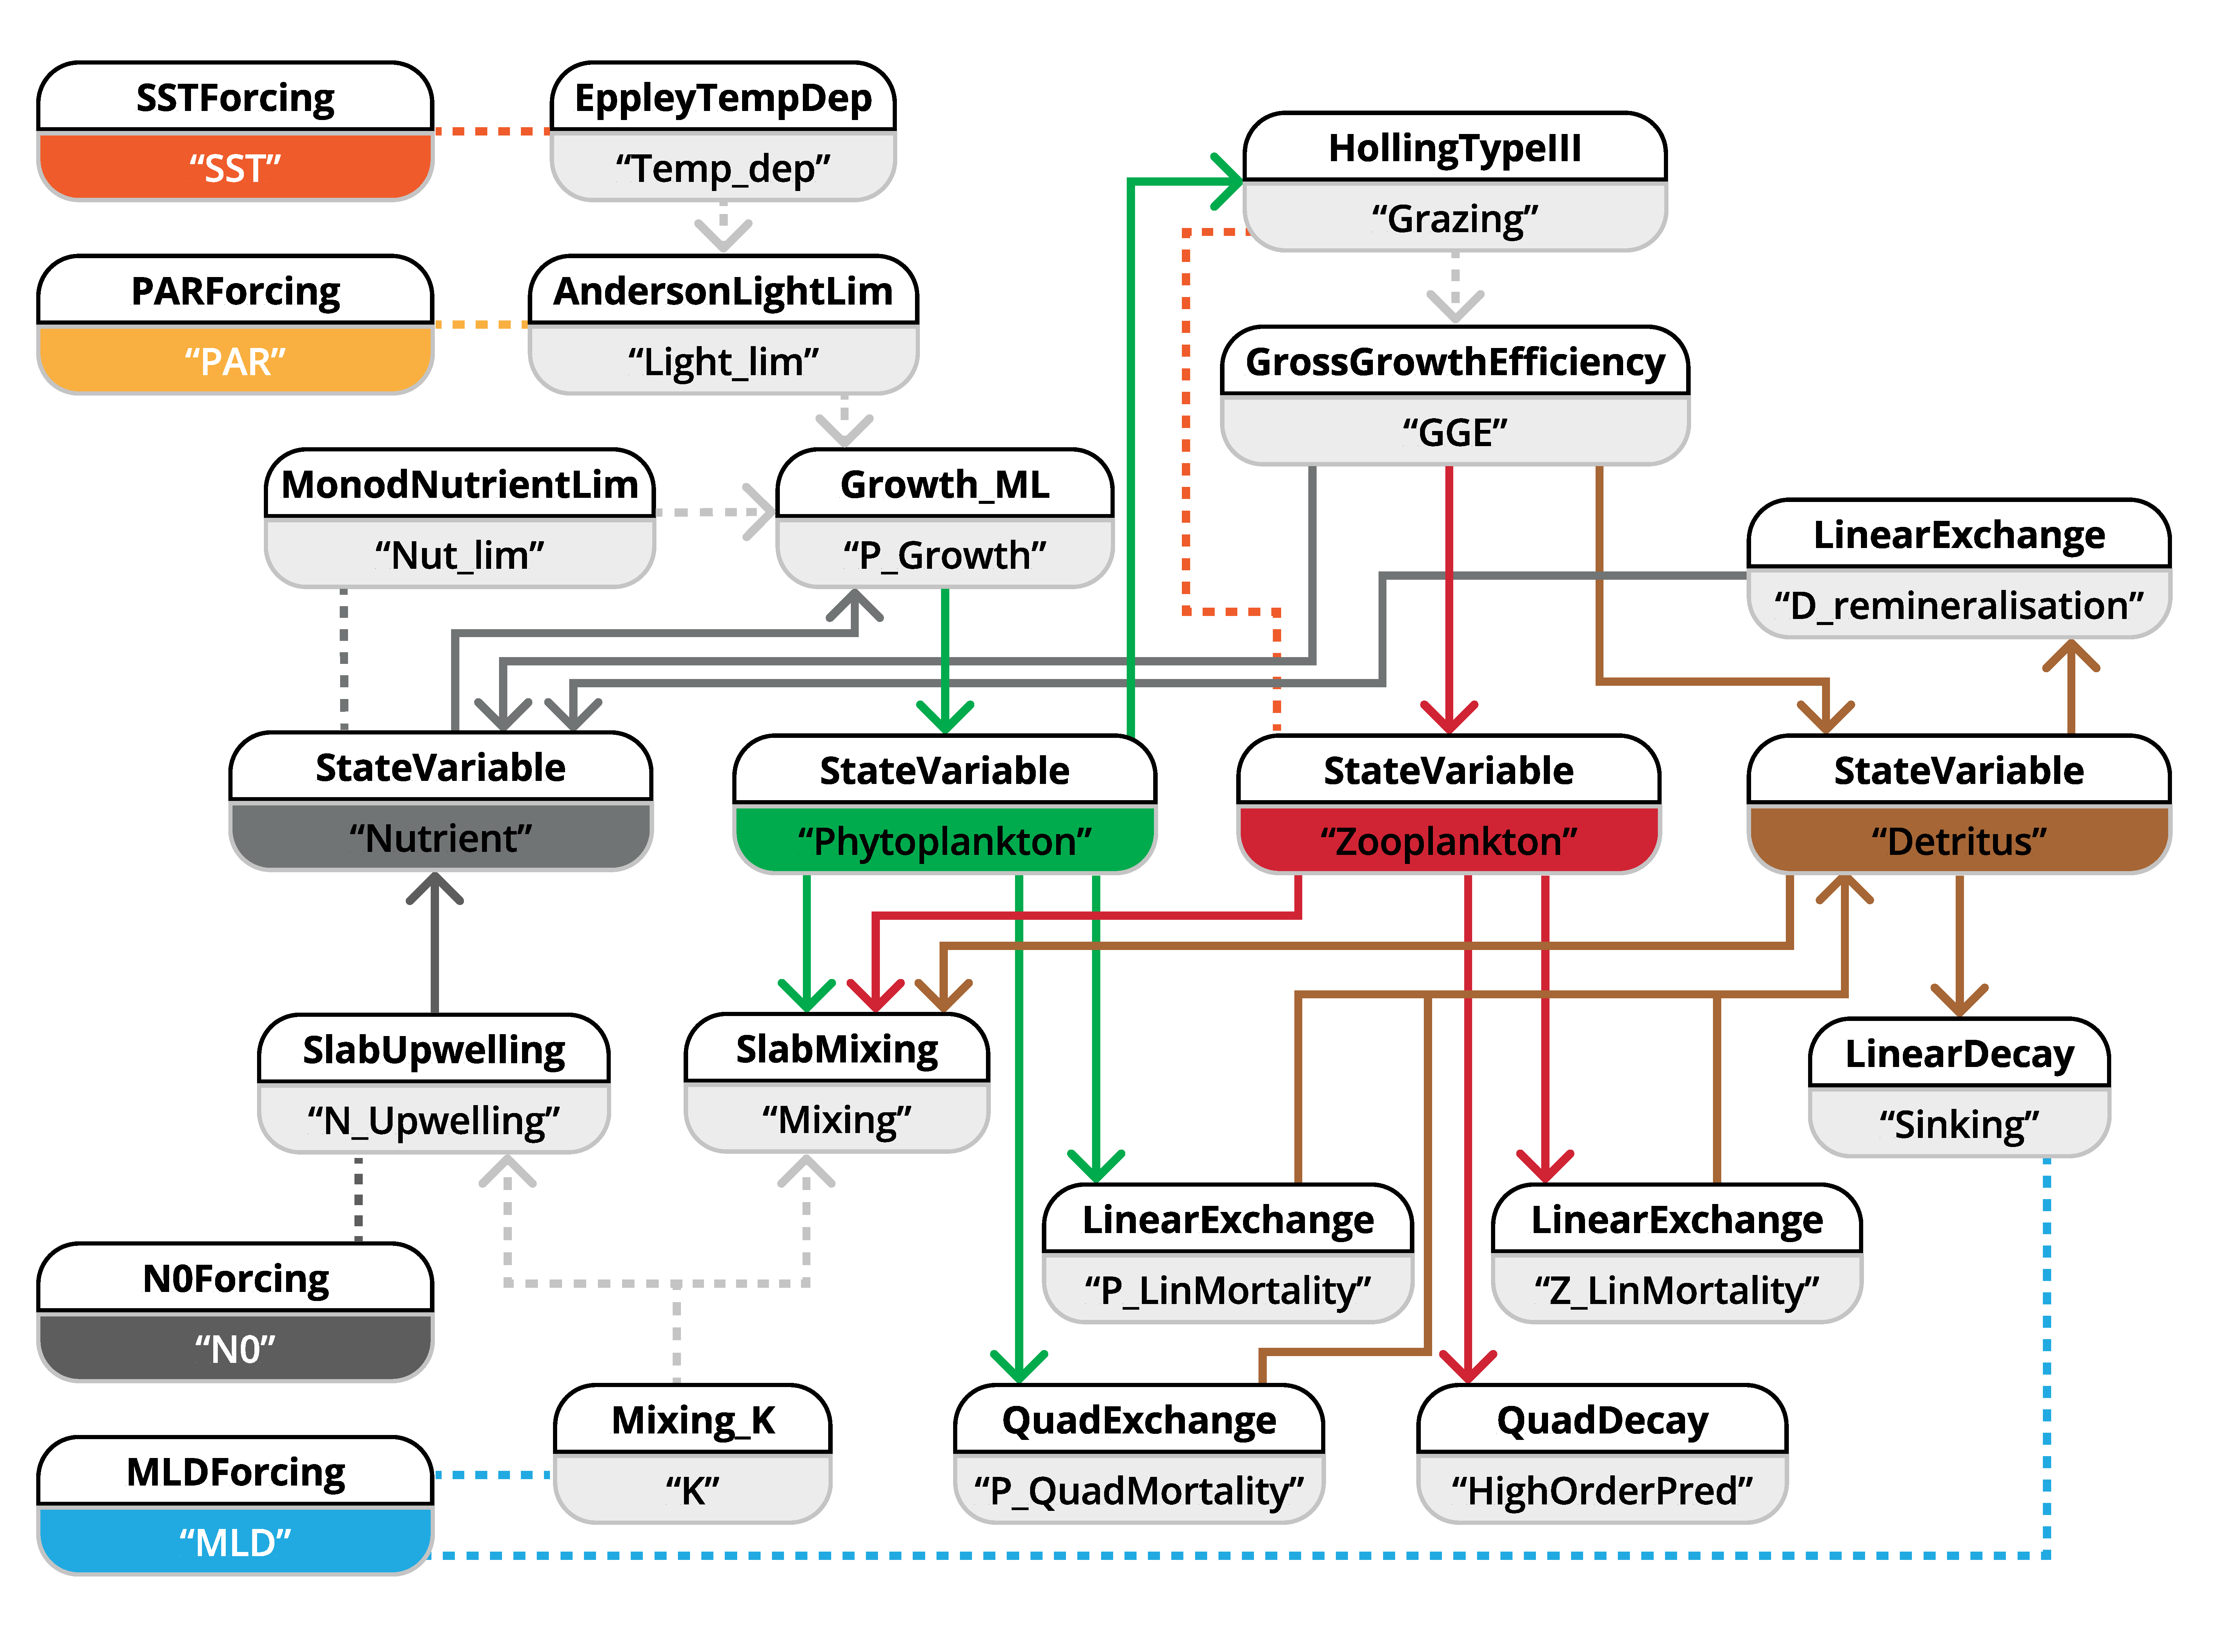
\includegraphics[width=15cm]{Figures/firstdraft_schematics/code_schematics/EMPOWER.pdf}
\caption{A schematic representation of how the NPZD model (application 2) is implemented in the XSO framework and included in the Phydra library. To simplify visualization, only the XSO components with their labels and links are shown. Each component consists of a number of variables, forcing, or parameters. Solid arrows indicate the flow of fluxes between state variables. Dashed arrows indicate fluxes passed along as group variables. Dashed lines connecting processes indicate variables and forcing passed along via their label.}
\label{Figure:CodeSchematics_2}
\end{figure*}

As shown for the previous model application, we first separate the model into state variables, forcing, and fluxes.  State variables include nutrient ($N$), phytoplankton ($P$), zooplankton ($Z$), and detritus ($D$). Forcing to the model are the upper mixed layer depth ($H$), nutrient concentration below the upper mixed layer ($N_0$), temperature in the upper mixed layer ($T$), and irradiance at surface ($I$). The model defines ten unique fluxes: Phytoplankton growth, zooplankton grazing, nutrient upwelling, mixing, sinking, remineralisation, and four mortality terms.

The ecological description of our model system is adapted from the EMPOWER model, however the technical implementation using the XSO framework is quite different from the procedural R script of \citet{Anderson2015c}. Instead of using hard-coded flags to choose different ecological formulations, the XSO component structure provides open modularity and interchangeability. The XSO framework defines functions irrespective of the specific time-step used for evaluation and logically separates the solving algorithm from the model code into the XSO backend. This allows formulate the model irrespective of the complex nested for-loop structure used in the original R implementation. Adding and removing state variables is also simplified in our framework because allocating resources and storing variables in model output is handled based on the components defined at model creation.

The amount of fluxes and interdependencies between the calculations in this application require a more elaborate component structure than in the chemostat. In model construction, we aim to find a balance between component refactoring and structural simplicity. Our goal is to allow for every ecologically relevant term to be exchangeable. For example, each growth-limiting term was defined by an individual component. The "group variable" feature of the XSO framework allows for such a setup. As long as a flux defined in a component matches the group label in another component, that individual flux can be used for calculating the bulk flux. The group variable can collect multiple fluxes to sum or multiply over, but it can also be used to split the calculation of a single flux between two components.

One particular example of this is the way we implemented a component calculating the mixing coefficient $K$, which is computed and passed along to calculate nutrient upwelling and the mixing fluxes of phytoplankton, zooplankton and detritus. Also, there is growth limitation, which is a multiplicative process of the growth limiting terms. Fluxes defined with a group label can in turn take a group variable as input, as was did with the temperature-dependent maximum photosynthetic rate, which is passed along to calculate light limitation and is used, in turn, to calculate the total growth flux. 

The model implementation and structure built from Phydra components in explained in more detail in Appendix \ref{Appendix:Implementation2}.
% Probably the forcing plot can go in the appendix?
%%f
\begin{figure*}[t]
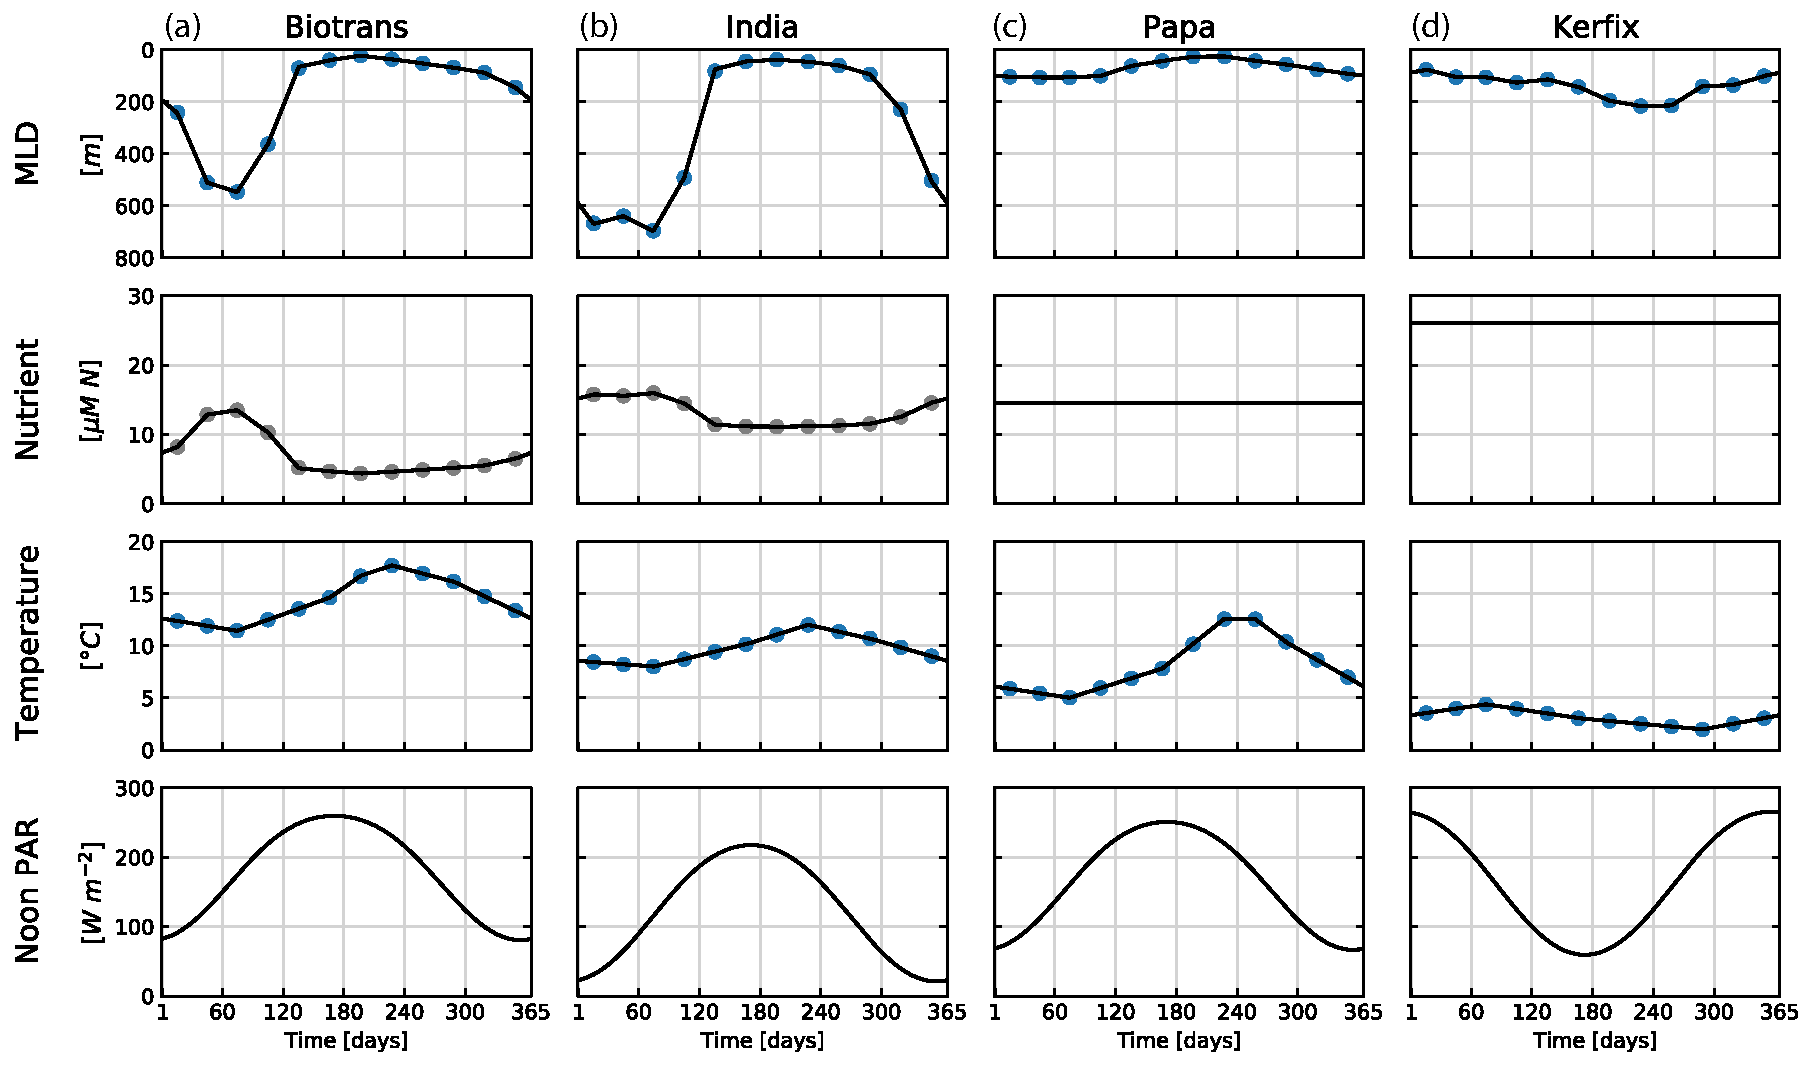
\includegraphics[width=15cm]{Figures/firstdraft_plots/02_EMPOWER_forcing.pdf}
\caption{Forcing corresponding to the four locations considered for the model application 2. Mixed Layer Depth ($H$), Nitrate below the Mixed Layer ($N_0$), irradiance at surface ($I$), and temperature averaged through the upper mixed layer ($T$). The mixed layer depth (MLD) and the temperature data are extracted from updated data sources corresponding to the original sources of Anderson et al. (2015). Nutrient forcing is a function of depth for locations Biotrans and India and a constant value for Papa and Kerfix. Irradiance is calculated as a function of latitude.}
\label{Figure:EMPOWERforcing}
\end{figure*}

We run the model in the same locations as \citet{Anderson2015c}: BIOTRANS, India, Papa, and KERFIX. Say briefly where each station is, and why it is relevant, eg "Papa is located in the subpolar North Pacific and has strongly seasonal cycles in X, Y, and Z". In each location, the NPZD slab model is forced by four corresponding environmental factors (Figure \ref{Figure:EMPOWERforcing}). 
The forcing for the Mixed Layer Depth ($H$) is taken from an updated version of the IFREMER MLD climatology  \citep{DeBoyerMontegut2004} including more data and using an optimized estimation of MLD (citation).
The nutrient concentration below the mixed layer ($N_0$) is calculated from a combination of the MLD climatology and depth-resolved climatology for nitrate in the World Ocean Atlas (WOA) 2018 \citep{Garcia2019WORLDSilicate}. The temperature of the mixed layer ($T$) was similarly calculated using the MLD climatology and the temperature data of WOA 2018 \citep{Locarnini2019WorldTemperature}.
The forcing for irradiance at surface ($I$) is calculated via a light submodel that employs trigonometric/astronomical equations to calculate light climatology for a location, given the latitude and cloud fraction as input parameters. The specific model used here and presented in \citet{Anderson2015c} was adapted from \citet{Shine1984ParametrizationAlbedo}.

As detailed in section \ref{Section:ComponentBuildingBlocks}, forcing from data needs to be interpolated to be compatible with an adaptive step-wise solver such as the SciPy's odeint algorithm used here. For comparability, we follow \citet{Anderson2015c} in linearly interpolating our forcing.

Following \citet{Anderson2015c}, the model is compared to seasonal data for nitrate within the upper mixed layer and chlorophyll concentration at all four stations. We used updated versions of the original data sources to retrieve the verification data. Nitrate within the upper mixed layer is calculated from a combination of the WOA 2018 nitrate data and the IFREMER MLD Climatology used for the $N_0$ forcing. Chlorophyll data is from MODIS Aqua chlorophyll climatology \citep{NASAGoddardSpaceFlightCenterOceanEcologyLaboratoryOceanBiologyProcessingGroup}. We did not follow the approach of taking a median year for chlorophyll data because the forcing is also climatology data and because we do not assume to be able to replicate particular biomass peaks of certain years. The climatological data follows the general pattern shown in the chlorophyll data used as verification data in the original paper.


The parameters used in model runs are adapted from \citet{Anderson2015c} and presented in Table \ref{Appendix:Table:EMPOWERparams}.

We used the batch dimension feature of the XSO model setup function, which we presented in section \ref{Section:Workflow:ModelSetup}. This feature allows to define a new dimension at model setup and to supply a list of values for a specific parameter. In our case, this additional dimension defines the four stations via the specific forcing and the parameters $V_P^{max}$, $\alpha$, $\mu_Z$ and $m_Z$, which are varied between locations \citep{Anderson2015c}. At runtime, the model is solved for each set of parameters in the supplied lists and outputs are returned in a single Xarray dataset. The model outputs for each station can then be easily retrieved via the supplied batch dimension label (in this case \texttt{"station"}).

\citet{Anderson2015c} included a detailed discussion of the treatment of light in a slab model. From the formulations presented in the original paper we considered two implementations. These are: the simple Beer's law, which parameterizes light attenuation with a single attenuation coefficient for the whole upper mixed layer, and the more elaborated piecewise description, which evaluates light attenuation in three discrete depth intervals within the upper mixed layer, with specific polynomial coefficients for each interval. Model results for both formulations are shown below.

\subsubsection{Results}
You'll want to add a, b, c, etc to subplots in this and all figures.
%%f
\begin{figure*}[t]
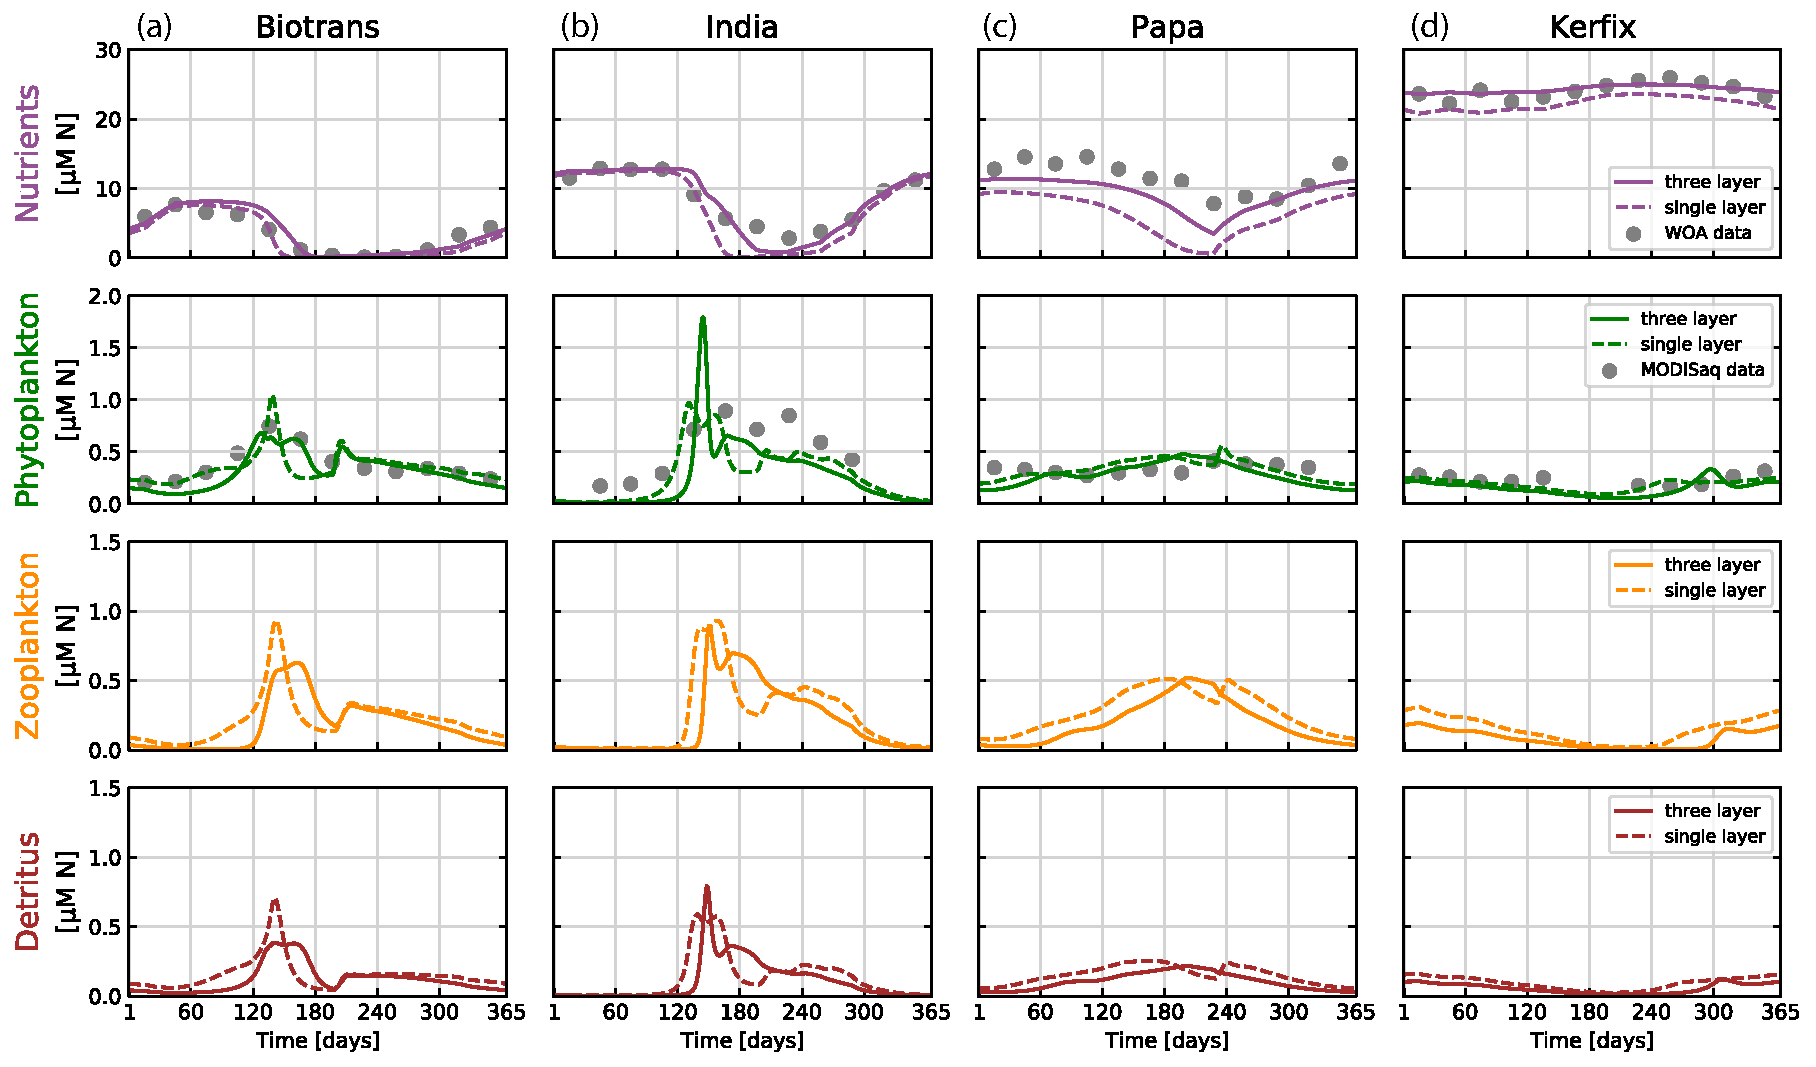
\includegraphics[width=15cm]{Figures/firstdraft_plots/02_EMPOWER_lightcomp.pdf}
\caption{Results of NPZD model (application 2) for locations A, B, C, and D. We show here the final year of a five-year run. The data for nitrogen in the upper mixed layer (dots) are taken from WOA 2018. Phytoplankton nitrogen biomass (dots) comes from the monthly chlorophyll climatology from MODIS Aqua; we converted chlorophyll to nitrogen biomass using fixed carbon:chlorophyll and carbon:nitrogen ratios of X and Y, respectively (provide citations, or explain this in the text where you mention MODIS).}
\label{Figure:ResultsEMPOWER}
\end{figure*}

Model outputs for all state variables in the corresponding stations are shown in Figure \ref{Figure:ResultsEMPOWER}. Our model outputs closely match the dynamics shown in the original paper \citep{Anderson2015c}. The model results obtained with light attenuated according to the three-layer formulation show a better agreement with the data, particularly for station Papa. This could be caused by a greater light limitation of phytoplankton growth, as nutrient draw-down during growth periods is consistently lower when compared to the simple Beer's law. These results show that our framework can recreate correctly the results of the model proposed by \citet{Anderson2015c} within a flexible and modular environment, which allows further experimentation and testing of different model structures.


\subsection{Model application 3: a size-based Nutrient-Phytoplankton-Zooplankton (NPZ) model}

The next example describes a size-structured plankton community model in an idealized physical setting. Cell or organism size is used in this type of model as a "master trait" which constrains organism traits and interactions \citep{Litchman2008}. This model structure is an adaptation of the ASTroCAT model \citep{Banas2011b}. Whereas Banas (2011b) considered model dynamics under variable forcing or with stochastic grazing parameters, we focus here on the basic setup under constant forcing. The model, defined in the context of a chemostat, features an allometric description of multiple size-classes for phytoplankton (growing on a single nutrient) and zooplankton (grazing on phytoplankton). While trophic interactions between size classes are highly resolved, other ecological processes are neglected (e.g. there is no detrital or regeneration pathways).  

The dimension functionality of the XSO framework and the built-in vectorisation of model equations constitute an ideal match for the implementation this model. Instead of defining state variables without dimensionality, as we did in the previous applications, we now add a dimension label to the \texttt{xso.variable} attribute within the component. This allows the user to initialise and use the variable as an array of size-classes, e.g. via \texttt{xso.variable(dims=("phyto"), ...)}. The number of size-classes is inherently variable and can be set at model setup. We showcase this feature by running the model with 2 to 50 size classes and comparing bulk phytoplankton biomass between runs.

\subsubsection{Description}
%%f
\begin{figure}[t]
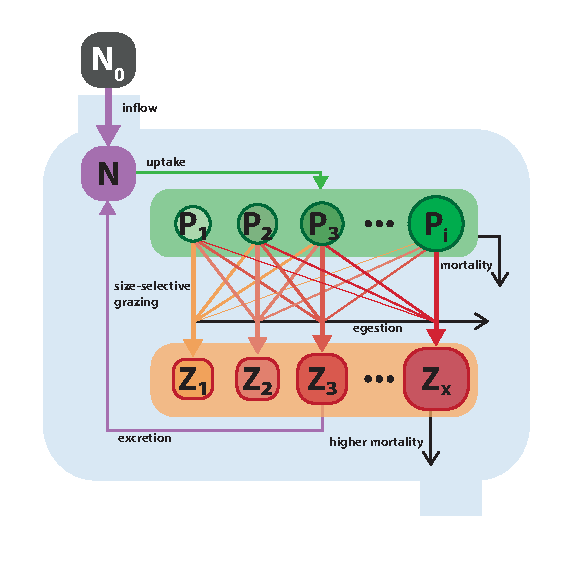
\includegraphics[width=8.3cm]{Figures/firstdraft_schematics/03_schematics_ASTroCAT.pdf}
\caption{Schematic of the size-resolved $NP_{i}Z_{j}$ trophic model. Model structure and parameterisation are adapted from \citet{Banas2011b}.}
\label{Figure:ModelSchematics_3}
\end{figure}

The model uses nitrogen as currency (state variables are expressed in units of $\mu mol$ N $m^{-3}$). The physical setting is analogous to a chemostat with constant nutrient inflow counterbalanced by permanent losses (outflow). The model describes a size-structured community of phytoplankton and zooplankton, which concentrations are expressed in terms of Equivalent Spherical Diameter (ESD). In line with \citet{Banas2011b}, we run simulations with 40 size classes of equally log-spaced $P$ (1 to 20 \unit{\mu m}), and 40 size classes of $Z$ (2.1 to 460  \unit{\mu m}). Additionally, we perform an experiment in which the number of size classes within these ranges is varied from 2 to 50. The model can be defined with any number of size classes within meaningful boundaries of allometric relationships. Size classes are denoted by the subscript $i$ for phytoplankton and $j$ for zooplankton.

%\subsubsection{Nutrient}
Model nutrient ($N$; units) is resupplied from an external source with concentration $N_0$ (units) delivered at a constant rate $f$ (units). In addition, a fraction of grazed biomass that is not assimilated by $Z$ (units) is returned to the nutrient pool. The only loss term for $N$ is phytoplankton nutrient uptake.

%\subsubsection{Phytoplankton}
Each phytoplankton size class $P_i$ grows according to Michaelis-Menten kinetics:

\begin{equation}
    \gamma_i^N =  \frac{N}{k_N^i + N} 
\end{equation}

where $\gamma_i^N$ is the limitation on phytoplankton growth due to nutrients, $k_N^i$ is the size-dependent half saturation nutrient concentration, and $N$ is the ambient nutrient concentration.

Phytoplankton loss due to natural mortality and excretion is described with the factor $m^P$ (units) that is scaled by the maximum intrinsic growth rate $\mu_{max}^i$ (units), so that $m^P \mu_{max}^i$ yields the specific mortality rate for each size class.

%\subsubsection{Zooplankton}
The grazing of the zooplankton size class $Z_j$ on the phytoplankton size class $P_i$ is calculated by
\begin{equation}
    G_P^{ij} = \mu_j^Z \ \frac{ \varphi_{ij} \cdot P_i }{ k_Z + \sum_{i}(\varphi_{ij} \cdot P_i) } \ Z_j
\end{equation}
where $\mu_Z^j$ is the size-dependent maximum ingestion rate, $k_Z$ is the half-saturation level and $\varphi_{ij}$ is the relative preference of $Z_j$ for $P_i$.

Prey preference is assumed to vary with phytoplankton size $size_{P}^i$ in a log-Gaussian distribution around an optimal prey size for each grazer $size_{opt}^j$.
\begin{equation}
    \varphi_{ij} = exp \left[ -\left( \ \frac{ log_{10}(size_P^i) - log_{10}(size_{opt}^j) }{ \Delta size_{P} } \right) \right]
\end{equation}
Where $\Delta size_{P}$ is the prey size tolerance parameter, in units of \unit{log_{10}(\mu m) ESD}, that controls the width of the Gaussian distribution.

Zooplankton growth is calculated as the product between total biomass grazed ($G_P$) and net production efficiency ($\epsilon$), for which values between 0.2 and 0.3 have been observed for a wide range of zooplankton \citep{Straile1997GrossGroup}. A fraction $f_{eg}$ of grazed biomass is assumed to be quickly excreted into $N$ and another fraction ($\epsilon$) that would feed into a detrital pool is permanently lost out of the system. Following \citet{Banas2011b}, the grazing fractions are split equally  so that $\epsilon = f_{eg} = 1/3$.

Zooplankton experience quadratic losses according to the parameter $m_{Z2}$. This term describes higher-order mortality and predation on zooplankton and is permanently removed from the system.

%\subsubsection{Model equations}
The temporal dynamics of the state variables are described by the following set of differential equations.

\begin{equation}
    \frac{d N}{d t} = 
    f \ N_0 % Nutrient mixing
    +  f_{eg} \ \sum_{j} \sum_{i} G_P^{ij} % Unassimilated grazing by Z
    - \sum_{i} ( \mu_{max}^i \ \gamma_i^N \ P_i) % Phytoplankton gains
\end{equation}

%PHYTOPLANKTON
\begin{equation}
    \frac{d P_i}{d t} =
    \mu_{max}^i \  \gamma_i^N \   P_i  % Phytoplankton gains
    - m_P  \ \mu_{max}^i \ P_i % Linear mortality
    - \sum_{j} G_P^{ij} % Z grazing
\end{equation}

%ZOOPLANKTON
\begin{equation}
    \frac{d Z_j}{d t} =
    \epsilon \ \sum_{i} G_P^{ij} % Assimilated grazing
    - m_{Z2} \ Z_j \ \sum_{j} Z_j  % Quadratic mortality
\end{equation}

Make sure to cite the table with model parameters and definitions. Same for Examples 1 and 2.

\subsubsection{Implementation}
%%f
\begin{figure*}[t]
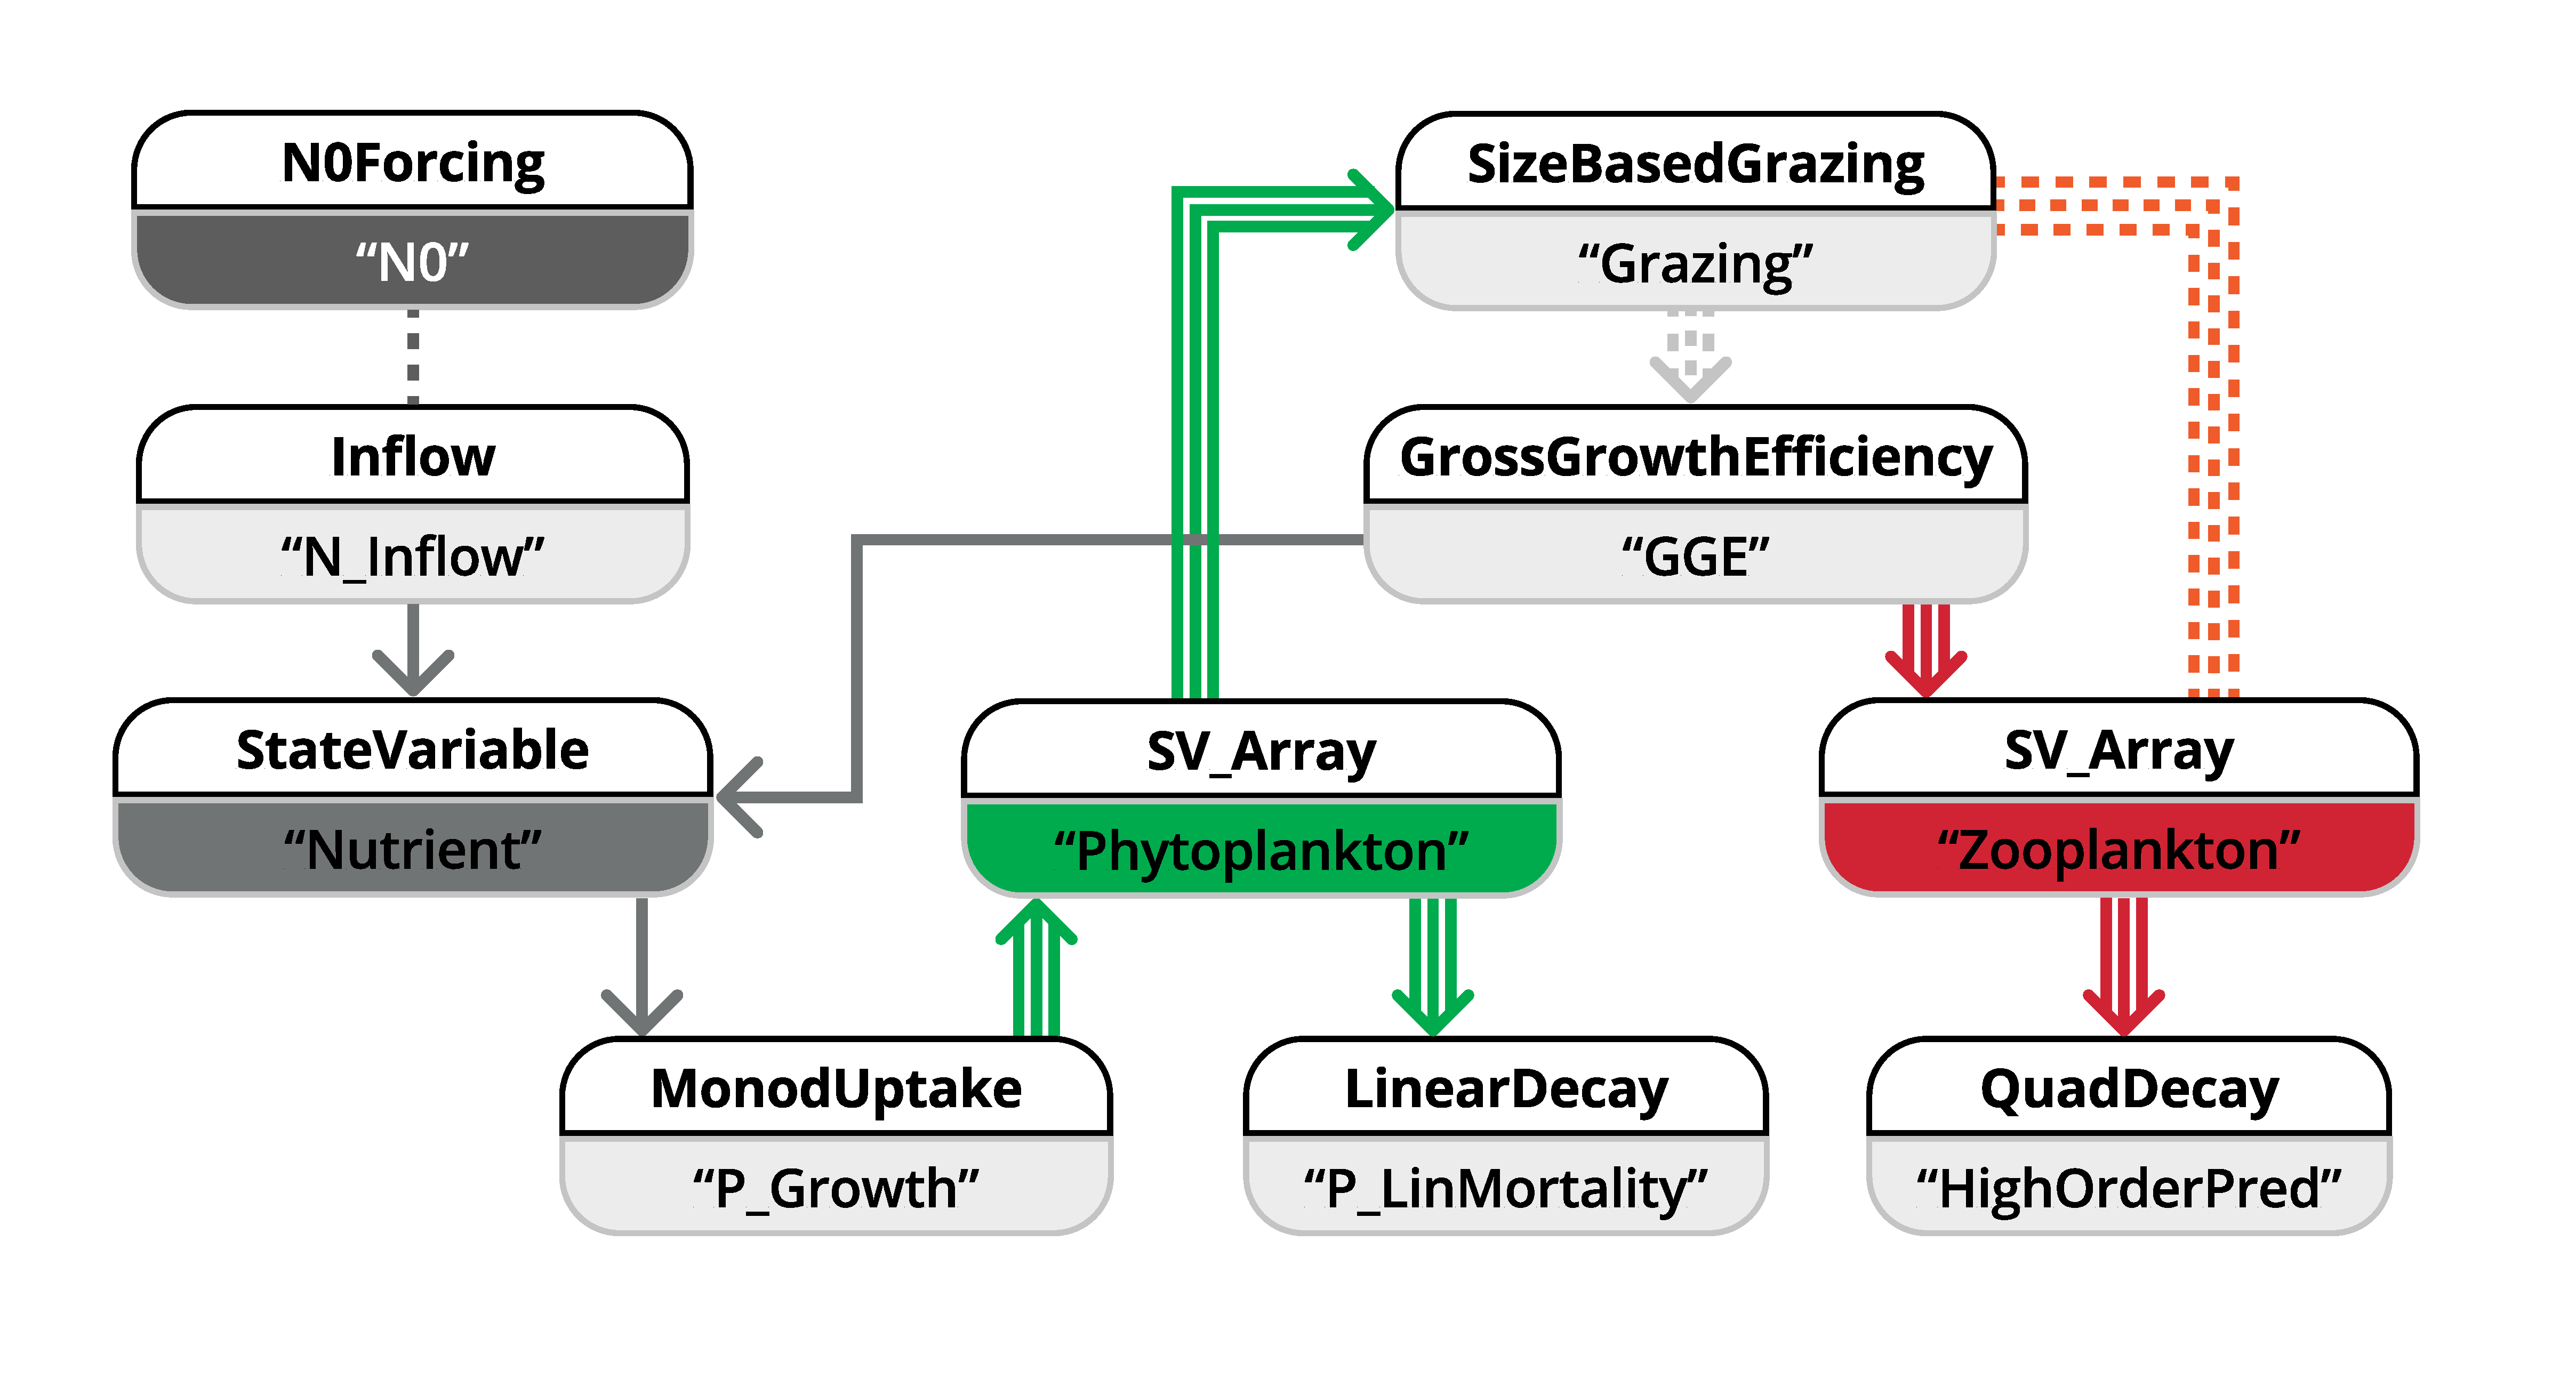
\includegraphics[width=15cm]{Figures/firstdraft_schematics/code_schematics/ASTroCAT.pdf}
\caption{A schematic representation of how model application 3 is implemented in the XSO framework and included in the Phydra library. For simplicity, only the XSO components with corresponding labels and links are shown. Each component consists of a number of variables, forcing, or parameters. Solid arrows indicate the fluxes between state variables. Dashed arrows indicate fluxes passed along as group variables. Dashed lines connecting processes indicate variables and forcing passed along via their label. Arrows with multiple lines indicate values with dimensions that are passed along.}
\label{Figure:CodeSchematics_3}
\end{figure*}

We separate the model into state variables, forcing, and fluxes. State variables are the nutrient ($N$), multiple size-classes of phytoplankton ($P_i$), and multiple size-classes of zooplankton ($Z_j$). The only forcing is the external nutrient input ($N_0$). At least 5 fluxes can be defined: The inflow of the external medium, $P_i$ growing on $N$, $Z_j$ grazing on $P_i$, and mortality terms for $P_i$ and $Z_j$.
The model was implemented using 10 XSO components (Figure \ref{Figure:CodeSchematics_3}). We simplify the schematic by only showing the components with their respective labels. A detailed description of each component can be found in the Phydra repository on GitHub.

The original ASTroCAT model was implemented with an interactive graphical user interface showing animations of model outputs. Our implementation in the XSO framework is technically quite similar to the original model code, with major differences being the modular component structure and the use of vectorization (instead of for-loops) to define functions computing the \textit{fluxes} acting on arrays of size-classes.

The implementation is presented in more detail in appendix \ref{Appendix:Implementation3}.

\citet{Banas2011b} presented a detailed analysis of model output for variable metrics of ecosystem complexity. We recreated a part of the analysis with a simple comparison of model dynamics for a variable number of phytoplankton and zooplankton size classes. The number of state variables can be varied at model setup by supplying a list of initial values with the desired dimensions. We ran the model for the range of 2 to 50 size classes.

\subsubsection{Results}
%%f
\begin{figure}[t]
\includegraphics[width=8.3cm]{Figures/firstdraft_plots/03_ASTroCAT_N50P50Z.pdf}
\caption{Nutrient concentration and plankton biomass under steady nutrient forcing obtained with model run resolving 50 phytoplankton and zooplankton size classes. Size classes are log-spaced in a range of 1 to 20 \unit{µ m} for phytoplankton and 2.16 to 420 \unit{µ m} for zooplankton. (a) Nutrient concentration over time. (b) Phytoplankton biomass by size class over 10 years of model time evolution. (c) Zooplankton biomass over the same period.}
\label{Figure:ResultsASTroCAT_1}
\end{figure}

Running the model with 40 size classes of phytoplankton and zooplankton recreates the dynamics presented by \citet{Banas2011b}. See Figure \ref{Figure:ResultsASTroCAT_1} for the time evolution of $N$, $P_i$ and $Z_j$ over a ten-year run. The size-resolved food-web shows oscillatory changes in biomass with periods from days to years. Describe what the banding means, and the relevance of this result to diversity and foodwebs. Add 2-4 sentences laying out the meaning of this model run.

%%f
\begin{figure}[t]
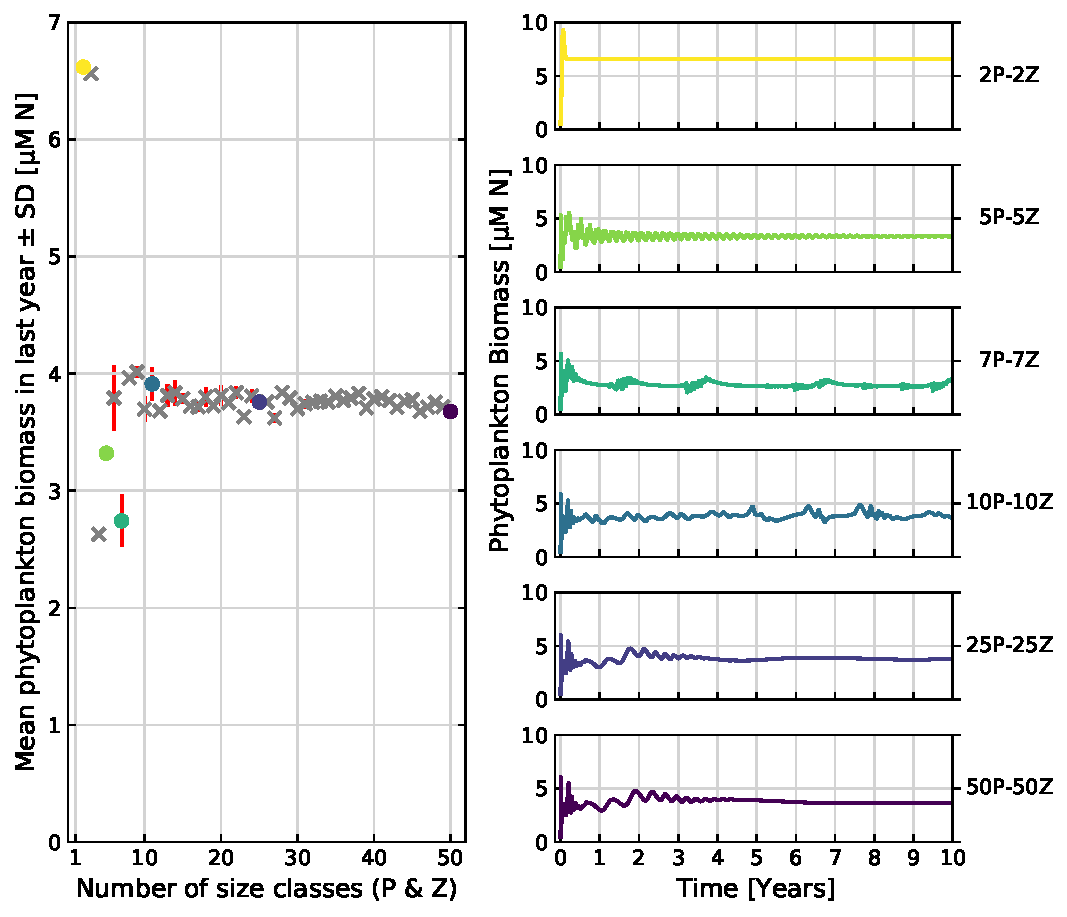
\includegraphics[width=8.3cm]{Figures/firstdraft_plots/03_ASTroCAT_sizeclassrange.pdf}
\caption{Comparative runs of X of varying number of size-classes. (a) Mean biomass of phytoplankton in the last year of a ten-year run for a range of 2 to 50 size classes of phytoplankton and zooplankton. Standard deviation is plotted in red. Grey crosses mark runs not otherwise shown, colored dots correspond to exemplary runs. (b) Exemplary model runs. The sum of phytoplankton biomass is shown over a ten-year run.}
\label{Figure:ResultsASTroCAT_2}
\end{figure}

Figure \ref{Figure:ResultsASTroCAT_2} shows the effect on bulk phytoplankton biomass when running the model with a variable number of size classes. A lower number of size classes (2-10) show highly variable outputs. Bulk dynamics seems to stabilize for numbers of size classes above 10. However, there are still deviations between runs in relation to the average phytoplankton biomass when more than 10 size classes are considered. The increased size resolution seems to reduce the perturbations carried on from initial model conditions, confirming the patterns observed by \citet{Baird2010IncreasingErrors}.


\section{Discussion}
% keep discussion simple! just mention a few important points!
% what is absolutely necessary?

\subsection{Structuring complex marine ecosystem models in a flexible framework}

I would add a paragraph about why XSO and Phydra are needed, and the overarching philosophy. 

% framework flexibility trade-off (design choices)
<Add a short topic sentence.> In creating a modelling framework, the design choices have a profound effect on both the flexibility and usability, with an inherent trade-off between these two aspects. In developing the XSO Framework and Phydra library, we went through multiple iterations of a self-contained framework that provides the user with a few options to customize pre-built models. The Phydra library provides users with fully functional models that can be set up and run via a simple user interface. These models remain fully accessible and modifiable through the underlying XSO framework.

% framework with Python backend and Python frontend
<Add a short topic sentence.> In contrast to available tools that allow building differential equation based models from a set of customisable building blocks through a graphical interface or other frameworks that utilise a custom scripting language (e.g. via YAML files), the Phydra and XSO frontend and backend are fully implemented in a single programming language: Python. This might require a higher initial effort for users unfamiliar to Python, but we argue that the effort is worth the wealth of functionality provided by the Python scientific ecosystem. The XSO model development workflow is similar to writing standard Python codes, with the added benefit of a set of modular Python objects and attributes that automatically handle model inputs and outputs and that allow to computationally construct and run the model. In common to other object-oriented modelling frameworks, functional model \textit{components} do not have to inherit from specific base classes. The functions defining \textit{forcings} and \textit{fluxes} within \textit{components} in XSO are not restrictive in their Python syntax and can make use of external Python packages, as long as the value that is finally supplied at model runtime is compatible with the chosen solver backend. Since XSO itself is a wrapper of Xarray-simlab without hiding the underlying functionality, this further expands the possibilities for custom applications and further development of the framework. The flexibility of the underlying framework should not dissuade users less interested in technical customisation, as the Phydra library provides fully functional pre-configured \textit{components} and \textit{model objects} that provide a solid foundation for marine ecosystem model development.

% flexibility in model construction
%The XSO framework is currently limited to model applications based on ordinary differential equations. With this limitation, conceptual marine ecosystem models still vary greatly in complexity. Our goal in developing the framework was to allow users to build models without restricting the level of complexity, in particular in relation to the number of state variables and model processes. This was implemented in the framework by providing \textit{variable types}, which directly correspond to the basic mathematical components of models based on ordinary differential equations (e.g. state variables, parameters, forcing, and partial equations). Every aspect of the model needs to be defined at the level of \textit{variable types}. Model \textit{components} can be flexibly constructed from the provided set of \textit{variable types} and wrap a logical component of the model as users see fit. There are no limitations to the number of \textit{variable types} used within a component and no limitations to the levels of \textit{group} variables linking components to define a single ecosystem process. State variables, forcing and parameters need to be initialised in one \textit{component} and can be referenced across the model. The system of differential equations is constructed from the \textit{fluxes} contained in the model \textit{components} via the supplied labels at model setup. These design choices make the effort required to construct models proportional to the desired model complexity and \textit{components} can be easily modified to more complex formulations. We hope that this will foster experimentation and inter-comparison of model performance at variable levels of complexity. 

Flexible Dimensionality! mention that
% Most of the above can actually go to the introduction!
% AND THEN HERE ACTUALLY DISCUSS THE DESING CHOICES AND COMPLEXITY of models; AND JUST THAT


\subsection{Current limitations of XSO and Phydra}
% XSO limitations
% XSO for ODEs only (by design)
- No "spatial" Dimension yet!
- Not making use of full xarray-simlab funcitonality
- "weak" linkages via strings

This first version of the XSO framework and Phydra library supports only mathematical models based on ordinary differential equations. There are no specific methods that help with setting up a system of partial differential equations, as would be needed for setting up a multi-dimensional model, but such functionality could be added in the future. Currently, there are no features implemented that go beyond constructing and solving a model. The framework structure would technically support advanced features for model introspection (e.g. printing the system of equations in LaTeX) or parameter optimization, but these features are still in an experimental phase and will be added to the XSO framework in later stages of development.

The first version of XSO implements a limited set of solver algorithms. These are a simple step-wise solver, an adaptive step-size solver optimized for solving system of ODES (Scipy's \texttt{odeint}). The simple step-wise solver is the only backend that currently supports multi model parallelism when executing multiple sets of parameters via the \textit{batch} dimensionality feature. None of the implemented solvers currently support single model parallelism and are thus not optimized for very large models (i.e. > 200 state variables).

% Current design paradigm rooted in flexible labeling to link components
<Add a topic sentence.> The high level of flexibility in the current version of XSO is rooted in the model backend that links the defined \textit{variable types} in separate \textit{components} via the supplied string labels at model setup. This design choice was made to allow easy reuse of \textit{components}. For example, a \textit{component} that defines a linear mortality flux acting on a single state variable could be implemented multiple times in a model to act on different state variables referenced via the associated label at model setup. This workflow allows for rapid prototyping, so that \textit{components} can be easily modified or exchanged and the routing of \textit{fluxes} can be modified even after creating the \textit{model object}. This is manageable for the presented use cases, but not ideal for very complex models that will require many labels to be supplied at model setup. Although this functionality is not yet built into the XSO user interface, implicit links between \textit{components} are technically possible via the underlying Xarray-simlab framework. This functionality can be implemented in future versions of XSO and should be considered for constructing models that aim at a high level of complexity for which the main goal is to extend and experiment on a specific model setup.

%\begin{comment}
% a comment for now, because I am not sure if this will be worked out in the first version of XSO or still an existing caveat
A caveat to the flexibility of \textit{components} is that currently the dimensions of \textit{variable types} need to be defined within a \textit{component} via a unique string label. The XSO framework checks at model setup that the dimension labels match in actual dimensionality across the model, e.g. that the mortality flux has the matching dimensionality to the referenced phytoplankton state variable that it acts upon. In order to allow full flexibility when exchanging \textit{components}, the user should be able to supply a specific dimension label at model setup, which is currently not supported by Xarray-simlab. A work-around is that the user modifies just that specific argument in the \textit{flux} within the \textit{component}.
%\end{comment}

% Phydra focus on simple physical settings for ecosystem models (no dimensionality yet!)



\subsection{Current usage and future developments}
% How to install and run Phydra?
- currently only installable via pip
- but we are working on providing it via conda

The Phydra library and the XSO framework are packages written in Python that can be easily installed via the Conda package management system. Conda is the ideal management system because it resolves and installs all necessary dependencies. Phydra and XSO are also available individually via the package installer for Python (pip). Detailed instructions about installation and resolution of dependencies can be found on the GitHub repository.

Since Python and the dependencies of Phydra are constantly developed, we provide instructions to install a fully compatible virtual environment with the Conda package manager separate from a user standard Python installation. For interactive coding and prototyping of models using Phydra, we recommend using the Jupyter notebook environment that is available via Conda. For more complex and larger model runs on servers, Python scripts are preferable.

% underyling packages are constantly developed, Phydra will grow with them
<Add a topic sentence.> The Xarray-simlab package that provides the basis for the XSO framework is a relatively young project and continuously under development, and this represents fruitful ground for developing and improving to the functionalities of Phydra and XSO. The Phydra library does not have to be tied to the XSO framework in future development. The Phydra library could be expanded to provide a functional Python interface to backend code specifically suited to marine ecosystem model applications.

% future feature development
The XSO framework in its current version allows building models quickly and dynamically from \textit{components} and provides a user interface to setup and run a model that is stored as a fully documented Xarray dataset. The Phydra library provides a set of \textit{components}, models and example applications that showcase the usability of the framework and provide a common library for marine ecosystem modelling applications. 

The features that we plan to develop next are: 

\begin{itemize}
    \item Methods for model introspection, such as printing the system of equations and visualising the model structure.
    \item Interface and methods for model parameter optimization.
    \item Custom methods to expand model dimensionality, to allow straight-forward definition of boundary condition and exchange between model compartments.
    \item An expanded solver backend that supports larger, multi-dimensional models.
\end{itemize}

The Phydra library of \textit{components} and \textit{model objects} could be expanded beyond the three applications presented here and would allow easy comparability and reproducibility of specific model applications, as demonstrated here.

Phydra and XSO are open-source projects. The source code is fully accessible on GitHub and can be freely used and modified according to a BSD-3 license. Contributions are welcome and in fact greatly appreciated. Users can contribute in many ways by reporting bugs, submitting feedback, contributing to the development of the code or the documentation. More information on how interested users can contribute to the project is provided in the online documentation.


%%% added Section label for editing purposes, later simply use \conclusions
\section{Conclusions}
%\conclusions  %% \conclusions[modified heading if necessary]
% Place this project in the wider open science ecosystem, summarize and conclude

%The Phydra library can be a reference and learning resource for scientists interested in marine ecosystem modelling, a starting point for scientific exploration, and a valuable tool for teaching. The XSO framework allows building ODE-based models in a flexible structure without restrictions to model complexity. The model development effort is proportional to the desired complexity of the model application, so users can quickly implement simple models.

Phydra is a Python library that offers fully configured marine ecosystem models and pre-constructed model building blocks (i.e. "components"), which can be combined to create custom configurations. The XSO package, which is the technical foundation of Phydra, provides a user-friendly interface and a modular modeling framework for building and solving computational models based on differential equations. The XSO framework grants users detailed control over state variables, parameters, forcing, and mathematical functions, making each defined model component interchangeable. Additionally, Phydra utilizes the Xarray dataset format for structuring model input and output, including metadata, allowing for easy storage, sharing, and analysis of data.

The Phydra library can be a reference and learning resource for scientists interested in marine ecosystem modelling, a starting point for scientific exploration, and a valuable tool for teaching. The XSO framework allows building ODE-based models in a flexible structure without restrictions to model complexity. The model development effort is proportional to the desired complexity of the model application, so users can quickly implement simple models.

We hope that 

This project aims to unify the computational tools used by scientists for data analysis and visualisation in Python with a functional, flexible, and open-source modelling framework. The package architecture is built on other open-source efforts (Xarray-simlab, Xarray, SciPy and NumPy to name a few) and provides a modular framework that could be further developed to provide an interface to more advanced domain-specific modelling frameworks such as Veros-BGCM or the FABM framework.

We presented three model applications of variable ecosystem complexity in zero-dimensional physical settings. These are contained in the first version of the Phydra library. A simple chemostat model of phytoplankton growing on a single nutrient showcases the workflow of implementing a model in the XSO framework in detail. The two following applications are implementations of previously published models that demonstrate the advanced functionality of the XSO framework. The second application is based on the EMPOWER model \citep{Anderson2015c}, a canonical open-ocean slab model that form the foundation of the field of marine ecosystem modelling. The third application is based on the ASTroCAT model \citep{Banas2011b}, which resolves complex trophic interactions within a size-resolved plankton model embedded in a simple physical flow-through setting. These three applications are contained in the Phydra library via their respective model \textit{components} and as fully assembled \textit{model objects}. Additionally, all scripts used to create the presented results are available in fully documented Jupyter notebooks in the model examples folder of the Phydra package. This should provide a foundation for users to start experimenting with the modelling framework. 

We hope Phydra and XSO contribute to the ongoing efforts in the marine ecosystem modelling community of developing more robust, transparent, and reproducible models, moving away from monolithic and inflexible codes to a model development process that is inherently collaborative. Both packages are open source and available under a BSD-3 license on GitHub.

%% END OF SECTION CONCLUSIONS









%% The following commands are for the statements about the availability of data sets and/or software code corresponding to the manuscript.
%% It is strongly recommended to make use of these sections in case data sets and/or software code have been part of your research the article is based on.

\codeavailability{TEXT} %% use this section when having only software code available


\dataavailability{TEXT} %% use this section when having only data sets available


\codedataavailability{TEXT} %% use this section when having data sets and software code available


\sampleavailability{TEXT} %% use this section when having geoscientific samples available


\videosupplement{TEXT} %% use this section when having video supplements available


\appendix


\section{Creating new components}  \label{Appendix:CreatingXSOComponent}

To implement ecosystem models beyond those included in the Phydra library, users can build custom \textit{components} from a set of \textit{variable types} provided by the XSO framework. Constructing a \textit{component} is as simple as writing a Python class, except that the framework greatly reduces the necessary boilerplate code (e.g. there is no need to define dunder methods such as \texttt{\_\_init\_\_}). The \textit{variable types} can be flexibly combined as attributes and function decorators within a class that is decorated with \texttt{@xso.component}. The decorator converts the class to a functional Xarray-simlab \textit{process} and registers the \textit{variable types} in the XSO backend.

The currently implemented \textit{variable types} in the XSO framework are presented below:
\begin{enumerate}
    \item \textbf{\textit{State variable}}: The class attribute \texttt{xso.variable} registers a time-dependent state variable with the following arguments currently available:
    \begin{itemize}
        \item \texttt{foreign}: A binary choice exists between defining the \textit{state variable} at model setup locally within the \textit{component}, or retrieving its value defined in another \textit{component}. These choices are given by the \texttt{foreign} argument available for \textit{state variables} and \textit{forcings}. The benefit to defining \texttt{foreign=True} is that a specific variable can be defined in a single component and referenced throughout the model. Additionally the variable can be flexibly modified by exchanging the \textit{component} that defines the referenced \textit{variable type} in the model. When a forcing or state variable defined as \texttt{foreign=False} (the default option) the user needs to supply a string label at model setup that uniquely identifies the variable within the model.
        
        \item \texttt{dims}: A \textit{state variable} can be implemented as a scalar (the default option) or as an array by supplying a string label for the \texttt{dim} argument. The label defines the variable dimension across the model at model setup and runtime.
        
        \item \texttt{list\_input}: XSO implements this feature to allow greater flexibility in setting up components that act on multiple variables in a similar manner. The list input feature can be activated via \texttt{list\_input = True} if the \textit{state variable} is defined as \texttt{foreign = True}. At model setup the user can supply a list of labels that are iterated over, calculating the specific flux acting on each supplied \textit{state variable}.
        
        \item \texttt{flux}: To define a specific mathematical function acting on the \textit{state variable}, a \textit{flux} function needs to be defined within the \textit{component}. Additionally, to create an implicit link between the defined \textit{state variable} and the \textit{flux}, the name of the \textit{flux} function is supplied to the \texttt{flux} argument.
        
        \item \texttt{negative}: If an argument was made to \texttt{flux}, the \texttt{negative} argument allows changing the mathematical sign of how the \textit{flux} affects the \textit{state variable}. The default is that the result of the \textit{flux} is added to the \textit{state variable}. If \texttt{negative=True}, the \textit{flux} will be subtracted.
        
        \item \texttt{groups}: The \texttt{groups} argument takes a string label that can be referenced in a \textit{group} variable in another \textit{component}. The \textit{group} variable assembles all \textit{state variables} (or \textit{forcings} and \textit{fluxes}) that share the same label across the model and can be used as an array of these values. This allows great flexibility in linking variables between \textit{components} to extend or refactor model processes.
        
        \item \texttt{description}: The argument allows passing a short string descriptor of the implemented variable that is included in the \textit{model object}, e.g. to clarifiy the purpose of the variable to a user. The description is available at all steps of the modeling workflow.
        
        \item \texttt{attrs}: The argument allows including more detailed metadata (e.g. units or citation) that will be included with the \textit{model setup} and model output Xarray datasets.
    \end{itemize}
    
    A \textit{component} can contain any number of \textit{state variables}. In the Phydra library we followed the design pattern that \textit{state variables} are defined within a simple \textit{component} that is reused with unique labels for each required variable. All other \textit{components} reference these \textit{state variables} via the \texttt{foreign=True} functionality.
    
    
    \item \textbf{\textit{Forcing}}: The class attribute \texttt{xso.forcing} registers an external time-varying parameter. It shares the \texttt{foreign}, \texttt{dims}, \texttt{groups}, \texttt{description} and \texttt{attrs} arguments with the \textit{state variable} attribute. Additionally a forcing needs to be supplied with the following argument:
    \begin{itemize}
        \item \texttt{setup\_func}: The argument has to be supplied with the name of a locally defined forcing setup function. This is a Python function defined within the \textit{component} that contains any necessary logic or computation for supplying the time-dependent forcing to the XSO backend. The setup function constructs and returns the actual forcing function, that takes model time as input and returns the value of the forcing during model runtime.
    \end{itemize}
    
    Constant forcings could be supplied via a single parameter to a \textit{flux}, but in the Phydra library constant forcings are generally implemented as \textit{forcing} variables, to allow easy exchange to variable forcings without having to modify other \textit{components} in model. 

    All variables and parameters defined within component can be used as arguments in both the setup function and the forcing function, e.g. to calculate station-specific forcing from a more general \textit{component}.
    
    If the forcing is based on data and not a mathematical function or constant value, it is necessary to perform some type of interpolation to supply the forcing to the model at flexible time steps. The interpolation would naturally happen within the setup function, where the choice of interpolation algorithm is up to the user. In Phydra we use \texttt{scipy.interpolate.splrep}, an algorithm to calculate the B-spline representation of a 1-D curve, in particular because it allows for periodic interpolation that is useful for yearly climatological forcing.
    
    \item \textbf{\textit{Parameter}}: 
    Model parameters can be added to a \textit{component} via the \texttt{xso.parameter} class attribute. It shares the \texttt{dims}, \texttt{description} and \texttt{attrs} arguments with the \textit{state variable} attribute. Any parameter defined as an attribute is available as an argument to the \textit{flux} and forcing setup functions within a \textit{component}. The specific value of the \textit{parameter} is supplied at model setup.
    
    \item \textbf{\textit{Group}}: Class attribute
    The \texttt{xso.group} class attribute allows creating a \textit{group variable} that aggregates multiple variables defined in other components. \textit{State variables}, \textit{forcings} and \textit{fluxes} provide a \texttt{groups} argument that can be supplied with a string label. By supplying the same string label to the \texttt{name} argument of the \textit{group} variable, all variables defined in other components that match the label are collected as a list. 
    This group variable can be used in the calculation of fluxes similar to any other locally defined \textit{variable type} within the same \textit{component}. This allows for flexibility in model setup and provides extensible of models, e.g. growth-limiting terms can be aggregated to a final component that calculates total flux and limiting terms can removed or added flexibly.
    
    \item \textbf{\textit{Flux}}: 
    The previous building blocks for state variables, forcings and parameters create the structure of the model, but when solved at this stage there would be no meaningful simulation. The basic building block of the system of differential equations that underpin an XSO model are \textit{fluxes}. A \textit{flux} is a Python function within a \textit{component} that takes the locally defined \textit{state variables}, \textit{forcings} and \textit{parameters} as input arguments and is decorated with \texttt{@xso.flux}. The decorator can be used as is or supplied with specific values for the \texttt{dims}, \texttt{groups}, \texttt{description} and \texttt{attrs} arguments. The \textit{flux} defines a mathematical function acting on state variables that can be directly linked to a \textit{state variable} via their \texttt{flux} argument or can be passed along to a \textit{group} variable and assigned to a \textit{state variable} in another \textit{component}.

    
\end{enumerate}

A \textit{component} can contain any number of \textit{variable types} as attributes, as well as helper functions or other custom attributes and methods. A complex flux can be broken down into multiple functions contained in the same decorated Python class. Components do not rely on inheritance, which improves code readability and maintainability. Due to the decorating function and translation process, backend is highly flexible and hides complexity from users who want to focus on the scientific questions. But as an open-source project, more advanced users can delve into the backend that can be modified for custom applications.


\section{Model implementation details}
- Below we explain the model structure built from Phydra components in more detail:


\subsection{Model use case 1} \label{Appendix:Implementation1}
We start model construction from the list of state variables, forcings and fluxes mentioned before. Below we list the model components with a short explanation to their functionality and go through the XSO variable types used within:
\begin{enumerate}
    \item \texttt{StateVariable} defines a state variable locally within the component, and is implemented twice, for nutrient and phytoplankton respectively.
    \begin{itemize}
        \item \texttt{var}: A \texttt{xso.variable} that registers the state variable at model creation. At model setup the variable requires two inputs: The specific label used throughout the model to reference this state variable in other components and the initial value of this state variable.
    \end{itemize}
    
    \item \texttt{ConstantForcing} creates and registers a constant forcing value, that can be referenced in other components. Here it is employed to create the forcing for the nutrient concentration ($N_0$).
    \begin{itemize}
        \item \texttt{forcing}: A \texttt{xso.forcing} that registers the forcing at model creation. The variable has to be initialized with a setup function within the same component. At model setup the specific forcing label used in the model has to be supplied ("N0" in this case).
        \item \texttt{rate}: A \texttt{xso.parameter} whose value is supplied at model setup and is used within the forcing setup function.
        \item \texttt{def forcing(time,*)}: This is a basic Python function defined within the component class, that is linked via its name to the forcing variable defined above. The asterisk is pseudo-code to reference the availability of all parameters defined in the component, specifically the \texttt{rate} parameter defined above. The setup function can include code to read or modify data, or calculate a specific time-dependent forcing. This forcing is then registered in the XSO framework, and will be called within the model backend when the forcing is referenced in other components.
    \end{itemize}
    
    \item \texttt{Inflow} is our first component that defines a flux, in this case the constant input of medium with nutrient concentration $N_0$ into our medium.
    \begin{itemize}
        \item \texttt{resource}: A \texttt{xso.variable} with the argument \texttt{foreign=True}. At model setup this variable requires a single input, which is the label of the state variable that should be affected by the fluxes defined in the component. The other arguments that are necessary for this is \texttt{flux="inflow"}, referencing the flux defined below. By default the flux is adding to the state variable, but this can be modified by passing the argument \texttt{negative=True} if so required.
        \item \texttt{forcing}: A \texttt{xso.forcing} with the argument \texttt{foreign=True}. Similar to the variable defined above, this forcing requires a label to the foreign forcing referenced here. It can be used as an argument in the flux function defined below.
        \item \texttt{rate}: A \texttt{xso.parameter} whose value is supplied at model setup and is used within the flux function below.
        \item \texttt{def inflow(*)}: A basic Python function decorated with \texttt{@xso.flux}. Through the flux argument supplied to \texttt{resource} it is linked via its name to the foreign state variable. The asterisk is pseudo-code to reference the availability of all parameters and forcings defined within the component, specifically we use the \texttt{rate} parameter and \texttt{forcing} defined above. This flux function consists of the basic mathematical calculation that defines the flux. For this simple constant input it calculates \texttt{forcing * rate} and adds that value to the state variable \texttt{resource}. With the labels and values supplied at model setup this flux returns $N_0 * 0.1$ at model runtime.
    \end{itemize}
    
    \item \texttt{MonodGrowth} is another component that defines a flux, in this case the uptake of nutrient and growth of phytoplankton based on Monod kinetics.
    \begin{itemize}
        \item \texttt{resource}: A \texttt{xso.variable} with the argument \texttt{foreign=True}. The flux \texttt{"uptake"} is linked via the \texttt{flux} argument with the option \texttt{negative=True} enabled. At model setup we supply the label \texttt{"N"}.
        \item \texttt{consumer}: A \texttt{xso.variable} with the argument \texttt{foreign=True}. The flux \texttt{"uptake"} is linked via the \texttt{flux} argument. At model setup we supply the label \texttt{"P"}.
        \item \texttt{halfsat}: A \texttt{xso.parameter} defining the half-saturation constant whose value is supplied at model setup and is used within the flux function below.
        \item \texttt{mu}: A \texttt{xso.parameter} defining the phytoplankton growth rate whose value is supplied at model setup and is used within the flux function below.
        \item \texttt{def uptake(*)}: This is Python function  decorated with \texttt{@xso.flux}. It is linked to the state variable defined as \texttt{resource} as negative term, and adds to the total flux of the state variable defined as \texttt{consumer} at model setup. The flux function returns a Monod function based on the values of \texttt{resource} and \texttt{consumer}, as well as the parameters \texttt{halfsat} and \texttt{mu} in the mathematical formulation $\mathit{mu} \frac{\mathit{resource}}{\mathit{halfsat}+\mathit{resource}} \mathit{consumer}$. With the labels supplied at model setup it returns $\mu \frac{N}{k_N+N} P$.
    \end{itemize}
    
    \item \texttt{Outflow} is final component defining a flux, specifically the outflow of both $N$ and $P$.
        \begin{itemize}
        \item \texttt{vars}: A \texttt{xso.variable} with the arguments \texttt{foreign=True} and \texttt{list\_input=True}. The flux is linked via \texttt{flux="outflow"} with the optional argument \texttt{negative=True} enabled. At model setup this variable requires a single input, which is a list of the labels of the state variables that are be affected by the flux defined in the component. Here we supply \texttt{["N","P"]}.
        \item \texttt{rate}: A \texttt{xso.parameter} whose value is supplied at model setup and is used within the flux function below.
        \item \texttt{def outflow(*)}: A basic Python function decorated with \texttt{@xso.flux}. The defined flux is computed individually for all state variables supplied to \texttt{vars}, but can be coded as a simple mathematical function with the framework handling the necessary routing. For this simple flux it calculates \texttt{vars * rate} and substracts that value from the state variables. With the labels and values supplied at model setup this flux returns $- N * 0.1$ acting on $N$ and $-P * 0.1$ acting on $P$ at model runtime.
    \end{itemize}
\end{enumerate}

The \texttt{Outflux} component shows off a feature of XSO, where fluxes affecting multiple variables in the same way allow for the definition of a list input to the variable at model setup. The flux function is computed for each supplied label in the list, and the XSO framework handles the routing of the flux values to their respective state variable. Particularly for models including many state variables, this feature simplifies the model creation and setup steps.


\subsection{Model use case 2} \label{Appendix:Implementation2}

The model was implemented using 23 separate model components as visualized in Figure \ref{Figure:CodeSchematics_2}. We chose to simplify the schematic by only showing the components with their respective labels, for a detailed view of each component please consult the Phydra repository on GitHub.

The model processes and their respective components are listed below, with a short description of their function and application in the model:

\begin{enumerate}
    \item State variables:
    \begin{itemize}
        \item \texttt{StateVariable}: This simple component defines a state variable within the XSO framework and was used to register the state variables $N$, $P$, $Z$ and $D$. At model creation the label of the component (e.g. "Nutrient") is supplied, while the label for the variable used to link fluxes to the variables (e.g. "N") is supplied at model setup.
    \end{itemize}
    
    \item Slab-ocean forcings:
    \begin{itemize}
        \item \texttt{MLDForcing}: The mixed layer depth forcing is read from a file, interpolated and supplied via the label \texttt{"MLD"} to the framework. 
        \item \texttt{N0Forcing}: The forcing for nutrient below the mixed layer is read from a file, interpolated and supplied via the label \texttt{"N0"} to the framework. 
        \item \texttt{PARForcing}: This component contains the light submodel, calculating irradiance climatology for the station locations.
        \item \texttt{SSTForcing}: The forcing for temperature within the mixed layer is read from a file, interpolated and supplied via the label \texttt{"SST"} to the framework.
    \end{itemize}
    
    \item Slab-ocean physics:
    \begin{itemize}
        \item \texttt{Mixing\_K}: From the forcing supplied via \texttt{MLDForcing} the mixing coefficient $K$ is calculated once and supplied to \texttt{SlabUpwelling} and \texttt{SlabMixing} via a group variable. $K$ is thus calculated only once per time-step for more efficient computation.
        \item \texttt{SlabUpwelling} calculates nutrient upwelling via the value of $K$ and the difference between the $N_0$ forcing and $N$. 
        \item \texttt{SlabMixing} employs the list-input functionality described in the first use case, and calculates the effect of mixing on $P$, $Z$ and $D$. Finally, 
        \item \texttt{SlabMixing} also receives the MLD forcing ($H$) from \texttt{MLDForcing} and calculates the sinking flux acting on $D$.
    \end{itemize}
    
    \item Phytoplankton growth: Temperature-dependent, light- and nutrient-limited growth of phytoplankton is another model process that was implemented with multiple linked components, to allow for greater flexibility.
    \begin{itemize}    
        \item \texttt{GrowthML} is the process that receives all the separate terms and calculates the net growth flux from a group variable. 
        \item \texttt{TempDepGrowth} calculates the maximum photosynthetic rate and passes the result along as a group variable to \texttt{SmithLightLim}. The temperature forcing ($T$) is supplied via the \texttt{SSTForcing} component.
        \item \texttt{SmithLightLim} calculates the integrated light limitation based on the maximum photosynthetic rate passed from \texttt{TempDepGrowth}. The forcing of irradiance at surface ($I$) is passed from the \texttt{PARForcing} component.
        \item \texttt{MonodGrowthLim} calculates nutrient-limitation dependent on the ambient nutrient concentration $N$ based on Monod kinetics. 
    \end{itemize}
    
    \item Zooplankton grazing: The grazing flux is set up via two components, that are linked via a group variable.
    \begin{itemize}    
        \item \texttt{HollingType3} calculates the total grazing fluxes that subtract from $P$ and $D$. [Explain Holling Type 3 shortly]. \texttt{HollingType3} was implemented with a list input for the resource variable, so that it would be simple to add or remove state variables from the zooplankton prey pool. The grazing preference is supplied as a list of the same dimension, where the order of values has to correspond to the order of supplied labels for the resource variable. 
        \item \texttt{GrowthGrowthEfficiency} receives the array of grazing fluxes ($P$ to $Z$ and $D$ to $Z$) and handles the routing of the total grazed biomass into three fractions, that are assimilated to $Z$, egested to $D$ and excreted to $N$ respectively.
    \end{itemize}
    
    \item Detritus remineralisation:
    \begin{itemize}
        \item \texttt{LinearExchange} takes a source and sink variable as input, as well as a rate parameter ($m_D$ in this case) and transfers that fraction from $D$ to $N$.
    \end{itemize}
    
    \item Mortality fluxes: Mortality fluxes can similarly be implemented using basic components from the Phydra library.
    \begin{itemize}
        \item \texttt{LinearExchange} calculates the linear mortality terms of $P$ and $Z$, both feeding into $D$. 
        \item \texttt{QuadExchange} implements quadratic phytoplankton mortality, as it feeds into $D$. 
        \item \texttt{QuadDecay} calculates higher-order mortality of zooplankton that is lost from the system.
    \end{itemize}
\end{enumerate}



%%% TWO-COLUMN TABLE
%
%t
\begin{table*}[t]
\caption{Model parameters used in runs for use case 2 for the four stations:}
\begin{tabular}{l c c c c c r}
\tophline
Parameter & Description & BIOTRANS & India & Papa & KERFIX & Units \\
\middlehline

$V_P^{max}$ & max. rate of photosynthesis at 0 \unit{\degree C} & 2.5 & 2.5 & 1.25 & 1.25 & \unit{g C (g chl)^{-1} h^{-1}}\\
$\alpha$ & initial slope of P-I curve & 0.15 & 0.15 & 0.075 & 0.075 & \unit{g C (g chl)^{-1} h^{-1}}\\
$k_N$ & half-sat. const: N uptake & 0.85  & 0.85  & 0.85  & 0.85 & \unit{µM \ N} \\
$m_P$ & linear P mortality & 0.015 & 0.015 & 0.015 & 0.015  & \unit{d^{−1}} \\
$m_{P2}$ & quadratic P mortality & 0.025 & 0.025 & 0.025 & 0.025 & \unit{(µM \ N)^{-1} d^{−1}} \\
$\mu_Z$ & Z max. ingestion rate & 1.0 & 1.0 & 1.25 & 2.0 & \unit{d^{−1}} \\
$k_Z$ & Z half-saturation for intake & 0.6 & 0.6 & 0.6 & 0.6 & \unit{µM \ N} \\
$\varphi_P$ & grazing preference: P & 0.67 & 0.67 & 0.67 & 0.67 & \\
$\varphi_D$ & grazing preference: D & 0.33 & 0.33 & 0.33 & 0.33 & \\
$\beta_Z$ & Z absorption efficiency & 0.69 & 0.69 & 0.69 & 0.69 &\\
$k_{NZ}$ & Z net production efficiency & 0.75 & 0.75 & 0.75 &  0.75 &\\
$m_Z$ & linear Z mortality  & 0.02 & 0.0 & 0.02 & 0.02 & \unit{d^{−1}} \\
$m_{Z2}$ & quadratic Z mortality & 0.34 & 0.34 & 0.34 & 0.34 & \unit{(µM \ N)^{-1} d^{−1}}  \\
$v_D$ & D linear sinking rate & 6.43 & 6.43 & 6.43 & 6.43 & \unit{m \ d^{−1}}\\
$m_D$ & D remineralisation rate & 0.06 & 0.06 & 0.06 & 0.06 & \unit{d^{−1}} \\
$\kappa$ & constant mixing parameter & 0.13 & 0.13 & 0.13 & 0.13 & \unit{m \ d^{−1}}\\
$\theta_{chl}$& constant mixing parameter & 75 & 75 & 75 & 75 & \unit{g \ g^{−1}} \\

\bottomhline
\end{tabular}
\label{Appendix:Table:EMPOWERparams}
\belowtable{These parameters were adapted from \citet{Anderson2015c}} % Table Footnotes
\end{table*}
%


\subsection{Model use case 3} \label{Appendix:Implementation3}
The model processes and their respective components are listed below, with a short description of their function and application in the model:

\begin{enumerate}
    \item State variables: 
    \begin{itemize}
        \item \texttt{StateVariable}: This is the same component used in the previous use cases. It registers the state variable for the ambient nutrient concentration ($N$). 
        \item \texttt{SVArraySize}: This is an extension of the \texttt{StateVariable} component, that additionally defines a dimension for the state variable and stores the array of sizes via a parameter. The supplied dimension label allows initializing a state variable as an array within the XSO framework, that is also represented in the Xarray data structure of the model setup and output. The number of values in the state variable array can be supplied flexibly at model setup by passing a list or array of that dimension as initial values. Across the model the framework will check that labelled dimensions share the same number of values. The label of the state variable (\texttt{"P"} and \texttt{"Z"} in this case) remains a single string and can be used across the model to reference the entire array. In this model we can use the same component (with the same dimension label) to register $P_i$ and $Z_j$, as the model was constructed for both of these to share the same number of dimensions.
    \end{itemize}

    \item Nutrient influx: 
    \begin{itemize}
        \item \texttt{ConstantForcing}: This component registers the external nutrient forcing ($N_0$) and is the same component that was applied in the first use case model.
        \item \texttt{Inflow}: The inflow flux is defined here, again this is the same implementation as in the first use case model. It adds to $N$ the flux defined as $N_0$ multiplied by a \texttt{rate} parameter. 
    \end{itemize}
    
    \item Nutrient uptake and phytoplankton growth: 
    \begin{itemize}
        \item \texttt{MonodUptake}: Similar to the nutrient influx components, this is a copy of the same component used in the first use case model, with the modification that we supply a dimension label to the \texttt{consumer} state variable and the parameters for \texttt{halfsat} and \texttt{mu}. We supply the label \texttt{"P"} for the \texttt{consumer} state variable. To set up the allometric parameters for the maximum growth rate and half-saturation constant, we calculate the parameters outside of the model definition and supply the values as a list at model setup.
    \end{itemize}
    
    \item Zooplankton grazing on phytoplankton: 
    \begin{itemize}
        \item \texttt{SizeBasedGrazing}: The grazing formulation for the multiple size classes of phytoplankton and zooplankton is the most complex function presented in our use cases. Care needs to be taken with proper handling of the dimensions within the function, but if it is done correctly the built-in vectorization of the XSO framework allows efficient calculation of the matrix-wise interaction for any number of size-classes. To improve the modularity of our implementation we split the calculation of the grazing matrix from the routing of the fluxes to their sources and sinks. This can be achieved via the group functionality of XSO, passing along the full matrix as a group variable to the \texttt{SizeBasedGrazing\_Fluxes} component. At model setup, the \texttt{SizeBasedGrazing} takes the label for resource and consumer, as well as the feeding preference matrix, the array of maximum ingestion rates and the single $k_Z$ parameter as input.
        \item \texttt{SizeBasedGrazing\_Fluxes}: This component receives the full matrix of grazing fluxes ($P_i$ over $Z_j$) as a group variable from the \texttt{SizeBasedGrazing} component and allocates the summed up fluxes to the sources and sinks of the grazing flux. Summing over $Z_j$ yields the array of grazing fluxes subtracting from $P_i$, while summing over $P_i$ and multiplying by the assimilation coefficient $\epsilon$ yields the array of grazing fluxes assimilated to $Z_j$. Summing over the entire matrix and multiplying by $f_{eg}$ yields the excreted biomass adding to $N$. At model setup, the component takes the respective labels of the state variables, as well as the parameters for $\epsilon$ and $f_{eg}$ as input.
    \end{itemize}
    
        \item Zooplankton and phytoplankton mortality: 
    \begin{itemize}
        \item \texttt{LinearDecayDim}: Linear mortality of phytoplankton can be defined with the same component employed in the first use case, with the modification that a dimension label is supplied as an argument to the flux and state variable. 
        \item \texttt{QuadDecayDim}: Similarly quadratic mortality of zooplankton is defined with a dimension label. The vectorization functionality allows defining the quadratic term as the sum of all zooplankton biomass, while still calculating over all zooplankton size classes.
    \end{itemize}
\end{enumerate}

The distribution of phytoplankton and zooplankton sizes are log-spaced. The \texttt{SVArraySize} \textit{component} registering the phytoplankton and zooplankton state variables takes the size range as parameter input, however this is only for documentation purposes. The allometric parameters are calculated via helper functions outside of model \textit{components} to allow maximum flexibility and reduce complexity of the specific model implementation.

Parameters were adapted from \citet{Banas2011b}, see table \ref{Table:usecase3parameters} for all used parameter values and allometric relationships.
\begin{table*}[t]
\caption{Parameters and allometric functions used in use case 3.}
\begin{tabular}{l c c r}
Parameter & Description & Value & Units \\
\tophline
$f$ & Flow rate of external nutrient & 1 & \unit{d^{-1}} \\
$N_0$ & External nutrient concentration & 1 & \unit{µM \ N} \\
$k_Z$ & Prey half-saturation constant & 3 & \unit{µM \ N}\\
$\Delta size_{P}$ & Prey size tolerance & 0.25 &  \\
$m_P$ & Mortality fraction of $\mu_{max}^i$ for $P_i$ & 0.1 & \unit{d^{-1}}\\
$\epsilon$ & Zooplankton growth efficiency & 0.33 & \\
$f_{eg}$ & Fraction of grazing egested & 0.33 & \\
\\

$\mu_{max}^i$ & Maximum growth rate of $P_i$ & $ 2.6 \left( \frac{size_i^{P}}{1\mu m} \right)^{-0.45}$  & \unit{d^{-1}} \\
$k_N^i$ & Nutrient half-saturation constant of $P_i$ & $ 0.1 \left( \frac{size_i^{P}}{1\mu m} \right)$ & \unit{µM \ N} \\

$\mu_Z^j$ & Maximum ingestion rate of $Z_j$ & $26 \left( \frac{size^i_{P}}{1\mu m} \right)^{-0.4}$ &\unit{µM \ N} \\

$size_{opt}^j$ &  & $0.65 \left( \frac{size_{P}^i}{1\mu m} \right)^{0.56}$ & \ \unit{µM \ N} \\

\bottomhline
\end{tabular}
\belowtable{Sources for allometric functions: \citep{Tang1995TheRespiration, Eppley1969HalfSaturationPhytoplankton, Hansen1997ZooplanktonRange, Hansen1994a}} % Table Footnotes
\label{Table:usecase3parameters}
\end{table*}
%


\noappendix       %% use this to mark the end of the appendix section. Otherwise the figures might be numbered incorrectly (e.g. 10 instead of 1).

%% Regarding figures and tables in appendices, the following two options are possible depending on your general handling of figures and tables in the manuscript environment:

%% Option 1: If you sorted all figures and tables into the sections of the text, please also sort the appendix figures and appendix tables into the respective appendix sections.
%% They will be correctly named automatically.

%% Option 2: If you put all figures after the reference list, please insert appendix tables and figures after the normal tables and figures.
%% To rename them correctly to A1, A2, etc., please add the following commands in front of them:

\appendixfigures  %% needs to be added in front of appendix figures

\appendixtables   %% needs to be added in front of appendix tables

%% Please add \clearpage between each table and/or figure. Further guidelines on figures and tables can be found below.



\authorcontribution{TEXT} %% this section is mandatory

\competinginterests{TEXT} %% this section is mandatory even if you declare that no competing interests are present

\disclaimer{TEXT} %% optional section

\begin{acknowledgements}
TEXT
\end{acknowledgements}




%% REFERENCES

%% The reference list is compiled as follows:

%\begin{thebibliography}{}

%\bibitem[AUTHOR(YEAR)]{LABEL1}
%REFERENCE 1

%\bibitem[AUTHOR(YEAR)]{LABEL2}
%REFERENCE 2

%\end{thebibliography}

%% Since the Copernicus LaTeX package includes the BibTeX style file copernicus.bst,
%% authors experienced with BibTeX only have to include the following two lines:
%%
\bibliographystyle{copernicus}
\bibliography{references.bib}
%%
%% URLs and DOIs can be entered in your BibTeX file as:
%%
%% URL = {http://www.xyz.org/~jones/idx_g.htm}
%% DOI = {10.5194/xyz}


%% LITERATURE CITATIONS
%%
%% command                        & example result
%% \citet{jones90}|               & Jones et al. (1990)
%% \citep{jones90}|               & (Jones et al., 1990)
%% \citep{jones90,jones93}|       & (Jones et al., 1990, 1993)
%% \citep[p.~32]{jones90}|        & (Jones et al., 1990, p.~32)
%% \citep[e.g.,][]{jones90}|      & (e.g., Jones et al., 1990)
%% \citep[e.g.,][p.~32]{jones90}| & (e.g., Jones et al., 1990, p.~32)
%% \citeauthor{jones90}|          & Jones et al.
%% \citeyear{jones90}|            & 1990



%% FIGURES

%% When figures and tables are placed at the end of the MS (article in one-column style), please add \clearpage
%% between bibliography and first table and/or figure as well as between each table and/or figure.

% The figure files should be labelled correctly with Arabic numerals (e.g. fig01.jpg, fig02.png).


%% ONE-COLUMN FIGURES

%%f
%\begin{figure}[t]
%\includegraphics[width=8.3cm]{FILE NAME}
%\caption{TEXT}
%\end{figure}
%
%%% TWO-COLUMN FIGURES
%
%%f
%\begin{figure*}[t]
%\includegraphics[width=12cm]{FILE NAME}
%\caption{TEXT}
%\end{figure*}
%
%
%%% TABLES
%%%
%%% The different columns must be seperated with a & command and should
%%% end with \\ to identify the column brake.
%
%%% ONE-COLUMN TABLE
%
%%t
%\begin{table}[t]
%\caption{TEXT}
%\begin{tabular}{column = lcr}
%\tophline
%
%\middlehline
%
%\bottomhline
%\end{tabular}
%\belowtable{} % Table Footnotes
%\end{table}
%
%%% TWO-COLUMN TABLE
%
%%t
%\begin{table*}[t]
%\caption{TEXT}
%\begin{tabular}{column = lcr}
%\tophline
%
%\middlehline
%
%\bottomhline
%\end{tabular}
%\belowtable{} % Table Footnotes
%\end{table*}
%
%%% LANDSCAPE TABLE
%
%%t
%\begin{sidewaystable*}[t]
%\caption{TEXT}
%\begin{tabular}{column = lcr}
%\tophline
%
%\middlehline
%
%\bottomhline
%\end{tabular}
%\belowtable{} % Table Footnotes
%\end{sidewaystable*}
%
%
%%% MATHEMATICAL EXPRESSIONS
%
%%% All papers typeset by Copernicus Publications follow the math typesetting regulations
%%% given by the IUPAC Green Book (IUPAC: Quantities, Units and Symbols in Physical Chemistry,
%%% 2nd Edn., Blackwell Science, available at: http://old.iupac.org/publications/books/gbook/green_book_2ed.pdf, 1993).
%%%
%%% Physical quantities/variables are typeset in italic font (t for time, T for Temperature)
%%% Indices which are not defined are typeset in italic font (x, y, z, a, b, c)
%%% Items/objects which are defined are typeset in roman font (Car A, Car B)
%%% Descriptions/specifications which are defined by itself are typeset in roman font (abs, rel, ref, tot, net, ice)
%%% Abbreviations from 2 letters are typeset in roman font (RH, LAI)
%%% Vectors are identified in bold italic font using \vec{x}
%%% Matrices are identified in bold roman font
%%% Multiplication signs are typeset using the LaTeX commands \times (for vector products, grids, and exponential notations) or \cdot
%%% The character * should not be applied as mutliplication sign
%
%
%%% EQUATIONS
%
%%% Single-row equation
%
%\begin{equation}
%
%\end{equation}
%
%%% Multiline equation
%
%\begin{align}
%& 3 + 5 = 8\\
%& 3 + 5 = 8\\
%& 3 + 5 = 8
%\end{align}
%
%
%%% MATRICES
%
%\begin{matrix}
%x & y & z\\
%x & y & z\\
%x & y & z\\
%\end{matrix}
%
%
%%% ALGORITHM
%
%\begin{algorithm}
%\caption{...}
%\label{a1}
%\begin{algorithmic}
%...
%\end{algorithmic}
%\end{algorithm}
%
%
%%% CHEMICAL FORMULAS AND REACTIONS
%
%%% For formulas embedded in the text, please use \chem{}
%
%%% The reaction environment creates labels including the letter R, i.e. (R1), (R2), etc.
%
%\begin{reaction}
%%% \rightarrow should be used for normal (one-way) chemical reactions
%%% \rightleftharpoons should be used for equilibria
%%% \leftrightarrow should be used for resonance structures
%\end{reaction}
%
%
%%% PHYSICAL UNITS
%%%
%%% Please use \unit{} and apply the exponential notation


\end{document}
